%% Zweiseitiges Layout
\documentclass[11pt,twoside,a4paper,fleqn,x11names]{report}
\usepackage[top=3cm, bottom=2.5cm, left=4cm, right=3cm]{geometry}

%% Schriftbild
\usepackage{lmodern}  % Latin Modern Zeichensatz
\usepackage[utf8]{inputenc}  % Unterstützung von Umlauten im Quelltext
\usepackage[T1]{fontenc}  % Korrekte Umlaute im PDF
\usepackage[english]{babel}  % Silbentrennung nach neuer Rechtschreibung
\renewcommand{\familydefault}{\sfdefault}  % Serifenlose Schrift
\usepackage{setspace}\onehalfspacing  % 1.5-facher Zeilenabstand
\renewcommand{\arraystretch}{1.5}  % 1.5-facher Zeilenabstand (Tabellen)
\setlength{\parindent}{0pt}  % Keine Einrückung am Beginn von Absätzen
\setlength\parskip{\medskipamount}
\usepackage{emptypage}
\usepackage{placeins} % plaziert figures in die richtige section
\usepackage{booktabs}
\usepackage{multirow}
\usepackage{siunitx}
\usepackage{subcaption}
\sloppy  % Weniger Silbentrennung

% Kopfzeile: Section auf linker Seite, Subsection auf rechter Seite
\usepackage{fancyhdr}
\pagestyle{fancy}
\renewcommand{\chaptermark}[1]{\markboth{#1}{}}
\renewcommand{\sectionmark}[1]{\markright{\thesection\ #1}}
\fancyhf{}
\fancyhead[LE,RO]{\small{\thepage}}
\fancyhead[LO]{\small{\rightmark}}
\fancyhead[RE]{\small{\leftmark}}
\renewcommand{\headrulewidth}{0.5pt}
\renewcommand{\footrulewidth}{0pt}
\fancypagestyle{plain}{%
  \fancyhead{}
  \renewcommand{\headrulewidth}{0pt}
}
%% Drawing:

\usepackage{tikz}
\usepackage{pgfplots}
\usepackage{tikzscale}
\usetikzlibrary{shapes,arrows,chains}
\usetikzlibrary{arrows.meta}
\usetikzlibrary{positioning}
\usetikzlibrary{math} %needed tikz library
\usetikzlibrary{backgrounds}
\pgfplotsset{compat=newest}
\pgfplotsset{
	colormap={whitered}{color(0cm)=(white); color(1cm)=(orange!75!red)}
}
\pgfplotsset{ignore zero/.style={%
		#1ticklabel={\ifdim\tick pt=0pt \else\pgfmathprintnumber{\tick}\fi}
}}
\usetikzlibrary{calc}

\newsavebox{\mybox}
\savebox{\mybox}{%
	\begin{tikzpicture}[background rectangle/.style={fill=white!45},show background rectangle, scale = 0.41]
	\begin{axis}[
	ymin=0, ymax=0.5,
    tick label style={font=\Huge},
    label style={font=\Huge},
	%minor y tick num = 3,
	area style,
	xlabel = {Fcst. Probability},
	ylabel = {Frequency},
	grid =major,
    major grid style={line width=.2pt,draw=gray!50},
	]
	\addplot+[ybar] plot coordinates { (0, 0.29) (0.1, 0.11) (0.2, 0.10) (0.3, 0.08) (0.4, 0.07) (0.5, 0.09) (0.6, 0.09) (0.7, 0.02) (0.8, 0.05) (0.9, 0.05) (1,0.10)};
	\end{axis}
\end{tikzpicture}
}

%\pgfmathdeclarefunction{gauss}{3}{%
%  \pgfmathparse{1/(sqrt(pow(#2,2)*2*pi))*exp(-(pow((#3-#1),2))/(2*pow(#2,2)))}%
%}
\pgfmathdeclarefunction{gauss}{4}{%A,mu,sigma,x
	\pgfmathparse{#1*(exp(-(pow((#4-#2),2))/(2*pow(#3,2))))}%
}

\pgfmathsetseed{12344}%
\pgfdeclarelayer{marx}
\pgfsetlayers{main,marx}
% A macro for marking coordinates (specific to the coordinate naming
% scheme used here). Swap the following 2 definitions to deactivate
% marks.
\providecommand{\cmark}[2][]{%
	\begin{pgfonlayer}{marx}
		\node [nmark] at (c#2#1) {#2};
	\end{pgfonlayer}{marx}
} 
\providecommand{\cmark}[2][]{\relax} 
%% Literaturverzeichnis (BibTex)
\usepackage{natbib}
\bibliographystyle{apalike}  % Layout des Literaturverzeichnisses

%% Verlinkung von Inhaltsverzeichnis, Bildern und Formeln
\usepackage[pagebackref]{hyperref}  % Verlinkung von URLs und Referenzen
\usepackage{color}  % Definition der Linkfarben
\definecolor{DarkRed}{rgb}{0.5,0,0}
\definecolor{Black}{rgb}{0,0,0}
\hypersetup{
  colorlinks,
  citecolor=Black,
  linkcolor=Black,
  urlcolor=Black}

\colorlet{lcfree}{Green3}
\colorlet{lcnorm}{Blue3}
\colorlet{lccong}{Red3}

%% Mathematikumgebung
\usepackage{array}
\usepackage{mathtools}
\usepackage{amsmath}
\usepackage{amssymb}  % Erweiterte Bibliothek mathematischer Symbole
\newcolumntype{M}[1]{>{\hbox to #1\bgroup\hss$}l<{$\egroup}}
%\usepackage{euler}  % Serifenlose Schrift in Formelumgebungen
\usepackage[makeroom]{cancel}  % Durchstreichen von Termen
\renewcommand{\deg}{\ensuremath{^{\circ}}}  % Grad Zeichen im Text
\renewcommand{\epsilon}{\varepsilon}  % Nutze richtiges Epsilon
\setcounter{MaxMatrixCols}{20}

\makeatletter
\newcommand\@brcolwidth{0.67em}
\newenvironment{brmatrix}{%
	\left[%
	\hskip-\arraycolsep
	\new@ifnextchar[\@brarray{\@brarray[\@brcolwidth]}%
}{%
	\endarray
	\hskip -\arraycolsep
	\right]%
}
\def\@brarray[#1]{\array{r*\c@MaxMatrixCols {M{#1}}}}
\makeatother

%% Grafikumgebungen
\usepackage{graphicx}  % Erweiterte Grafikumgebung
\usepackage{float}  % Automatische Positionierung von Bildern
\usepackage{subcaption}  %  Bildunterschriften für subfigures

%% Formeln, Bilder und Tabellen pro section nummerieren
\numberwithin{equation}{chapter}
\numberwithin{figure}{chapter}
\numberwithin{table}{chapter}

%% Listenumgebung
\usepackage{enumerate}
\usepackage{textcomp}  % Korrekte serifenlose Aufzählungszeichen

%% Farbige Umrahmungen
\usepackage{framed}
\definecolor{shadecolor}{rgb}{0.9,0.9,0.9}

%% Blindtext zum Testen des Layouts
\usepackage{blindtext}

%% Inhalt der Titelseite


%%%%%%%%%%%%%%%%%%%%%%%%%%%%%%%%%%%%%%%%%%%%%%%%%%%%%%%%%%%%%%%%%%%%%%
\setcounter{section}{0}
\begin{document}
	\thispagestyle{empty}
	\begin{center}
		\hspace*{0pt}\vfill
		\begin{Huge}
			Probabilistic Radar-Based Precipitation Nowcasting
		\end{Huge}
		\vfill
		\begin{minipage}{0.5\textwidth}
			\centering
			%\begin{flushleft}
				\begin{large}
					Master thesis by
				\end{large}
				\\\vspace{0.5cm}
				\begin{huge}
					Simon Michel
				\end{huge}
			%\end{flushleft}
		\end{minipage}
		\vfill
		
		\begin{minipage}{0.5\textwidth}
			\centering
			%\begin{flushleft}
				\begin{large}
					%Matrikelnummer: 6353359\\
					Universität Hamburg\\
					Fachbereich Geowissenschaften
				\end{large}
			%\end{flushleft}
		\end{minipage}
		\vfill
		
		\begin{minipage}{0.5\textwidth}
			\centering
			%\begin{flushleft}
				\begin{large}
					%Matrikelnummer: 6353359\\
					Erstgutachter: Dr. Marco Clemens\\
					Zweitgutachter: Prof. Dr. Felix Ament
				\end{large}
			%\end{flushleft}
		\end{minipage}
		\vfill
		\begin{minipage}{0.5\textwidth}
			\centering
			%\begin{flushleft}
				\begin{large}
					Hamburg, \today
				\end{large}
			%\end{flushleft}
		\end{minipage}
		\vfill
	\end{center}
	
	\newpage
	\thispagestyle{empty}
	\null
	\vfill
	Master thesis im Fachbereich Geowissenschaften der Universität Hamburg\\
	Thema der Arbeit: \glqq Probabilistic Radar-Based Precipitation Nowcasting\grqq
	
	
\newpage
\renewcommand{\abstractname}{\huge \flushleft Abstract}
\begin{abstract}
\null
\end{abstract}
\thispagestyle{empty}
\pagestyle{empty}
\tableofcontents
\listoffigures
\listoftables
\newpage\pagestyle{fancy}
\chapter{Introduction}
\pagenumbering{arabic}
\chapter{Meteorological Forecasting}
People always had the desire to forecast weather conditions. Until modern times the forecasts were based on local weather observation, folklore and rule of thumb. With the development of telecommunication the modern age of weather forecasting began \citep{Moore}. After \cite{Sene2009} and \cite{Pierce12} meteorological forecasting techniques nowadays can be generally divided into 3 categories:
\begin{itemize}
	\item Nowcasting - weather forecasting for up to 6 hours based on the current meteorological state of the atmosphere. Observations can include local weather radars, weather stations and satellite measurements.
	\item Numerical weather prediction (NWP) - NWP models utilize prognostic mathematical models of the atmosphere and oceans to predict the future state of the atmosphere based on current weather observations.
	\item Statistical methods - use statistical techniques, like regressions to estimate future conditions.
\end{itemize}
The listed meteorological forecasting techniques show skill on different timescales due to their model characteristics (Figure \ref{fig:prognosisquality}). Nowcasting relies on the extrapolation of observation data of satellites, radars and other measurements. This results in a high forecasting skill for short lead times of the forecast. Since nowcasting does not use prognostic equations and the forecast relies on the initial data the forecast quality quickly falls off with time. NWP use four-dimensional models of the atmosphere to predict future meteorological states. Due to the nature of NWP, caused by the data assimilation and the initialization of the model.
\section{Nowcasting}
\label{chap:nowcasting}
Nowcasting aims to estimate a future state of the atmosphere, such as clouds and storms, based on their current location, track, speed and the rate of their growth or decay. Nowcasting techniques are mostly used with weather radar applications but are also applied to satellite observations of clouds or thunderstorms, and are used in forecasting for tropical cyclones, hurricanes and typhoons.\\
In combination with weather radar data the aim of nowcasting is to estimate the development of storms, how they move and evolve in the next few hours. This is based on its present and recent location, extend, speed and track. The accuracy of forecasts depend on the local climatological conditions and topography, the type of precipitation event and the resolution and range of the weather radar data. For widespread frontal precipitation events nowcasting methods show skill for maximum lead times of up to 3-6 hours. Lead time for convective events are much shorter due to their short lifetimes \citep{Sene2009}.
\begin{figure}[!htbp]
	\centering
	\begin{tikzpicture}[
			>=triangle 60,              % Nice arrows; your taste may be different
			]
	\begin{axis}[
	axis x line=center,
	axis y line=center,
	xtick={0,3,6,9,12,15,18},
	ytick=\empty,
	xticklabels={0,6,12,18,24,30,36},
    ylabel near ticks,
	xlabel near ticks,
	xlabel={Lead time of forecast in hours},
	ylabel={Quality of forecast},
	xmin=0,
	ymin=0,
	xmax=19.5,
	ymax=8.5
	]
	\draw[thick] (0,8) .. controls (3.5,6) and (4,1.5) .. (6.5,0.5);
	\node at (12,7.5) [text width=5cm] {Extrapolation of the current atmospheric state using radar observations};
	\draw [<-] (2.5,6.3)--(4.5,7.5);
	
	\draw[thick] (0,4) .. controls (4,5) and (6,3) .. (11,1.8);
	\node at (11.5,5.5) [text width=5cm] {Mesoscale NWP model};
	\draw [<-] (4.5,4.1)--(6,5);
	
	\draw[thick] (3.2,0.3) .. controls (9,1.5) and (10.5,3.3) .. (19.5,1);
	\node at (13.2,4) [text width=5cm] {Synoptic-scale NWP model with Model Output Statistics};
	\draw [<-] (12.3,2.3)--(13.8,3.3);
	\end{axis}
	\end{tikzpicture}
	\caption{A schematic showing the quality of weather forecasts, defined by their accuracy and the achievable detail, as a function of lead time. Created after \cite{Pierce12} and \cite{Browning1980}.}
	\label{fig:prognosisquality}
\end{figure}\\
The development of nowcasting began with simple advection or extrapolation of precipitation. The clouds or storms were merely translated based on their current speed and direction. First applications of this technique were done by \cite{hilst1960} and \cite{Noel}. An important conclusion found in these early demonstrations was the positive correlation between the size of precipitation features and their predictability. Small features tend to have a shorter lifetime than large features. Small scale features have a typical lifetime of less than 30 minutes \cite{Sene2009}.

\section{Fieldbased}
\section{Cellbased}
\section{Probabilistic Nowcasting}
\chapter{Data}
\label{chap:data}
\section{DWD Radar Data}
The Deutscher Wetterdienst (DWD) operates a network of 17 polarimetric C-band Doppler radar systems which cover Germany (Figure \ref{fig:radarnetwork}). From this network the data from the Boostedt radar is used. The position of the Boostedt radar is 54.0055°\,N and 10.04683°\,E (red marker in Figure \ref{fig:radarOverview}). The DWD uses radars of the type 'DWSR/5001/SDP/CD' from the company EEC. With a frequency of 5600 - 5650\,MHz and a wavelength of approx. 5.3\,cm the radars operate in the C-band. As polarimetric Doppler radars the radars use horizontally and vertically polarized electromagnetic waves to measure the  reflectivity of hydrometeors. Since hydrometeor classification is not needed only the horizontally polarized waves are considered. \\
In this thesis only data from the precipitation scan of the DWD radar is used. This precipitation scan operates at the lowest elevation angle possible following the horizon line. It has a range of 150\,km and a range resolution of 250\,m at a angular resolution of 1\deg. The precipitation scan is performed every 5 minutes. From the total precipitation scan of the Boostedt radar (red circle in Fig. \ref{fig:radarOverview}) only a square with a edge length of 100\,km with Hamburg as centre is used (blue square). The technical specifications of the DWD radars are listed in Table \ref{tab:radarspec}.\\
For the post-processing and quality controlling of the radar data the DWD has developed a software package called 'Polarimetric Radar Algorithms' (POLARA). The radar data quality checking is done in two steps. First radar signal processing and then post-processing. In the signal processing several filters and thresholds are set to reduce undesired echoes and eliminate some  of the clutter \citep{Werner2014}. The DWD radar data used in this thesis is only quality controlled by the signal processing.
\begin{figure}[!htbp]
	\centering
	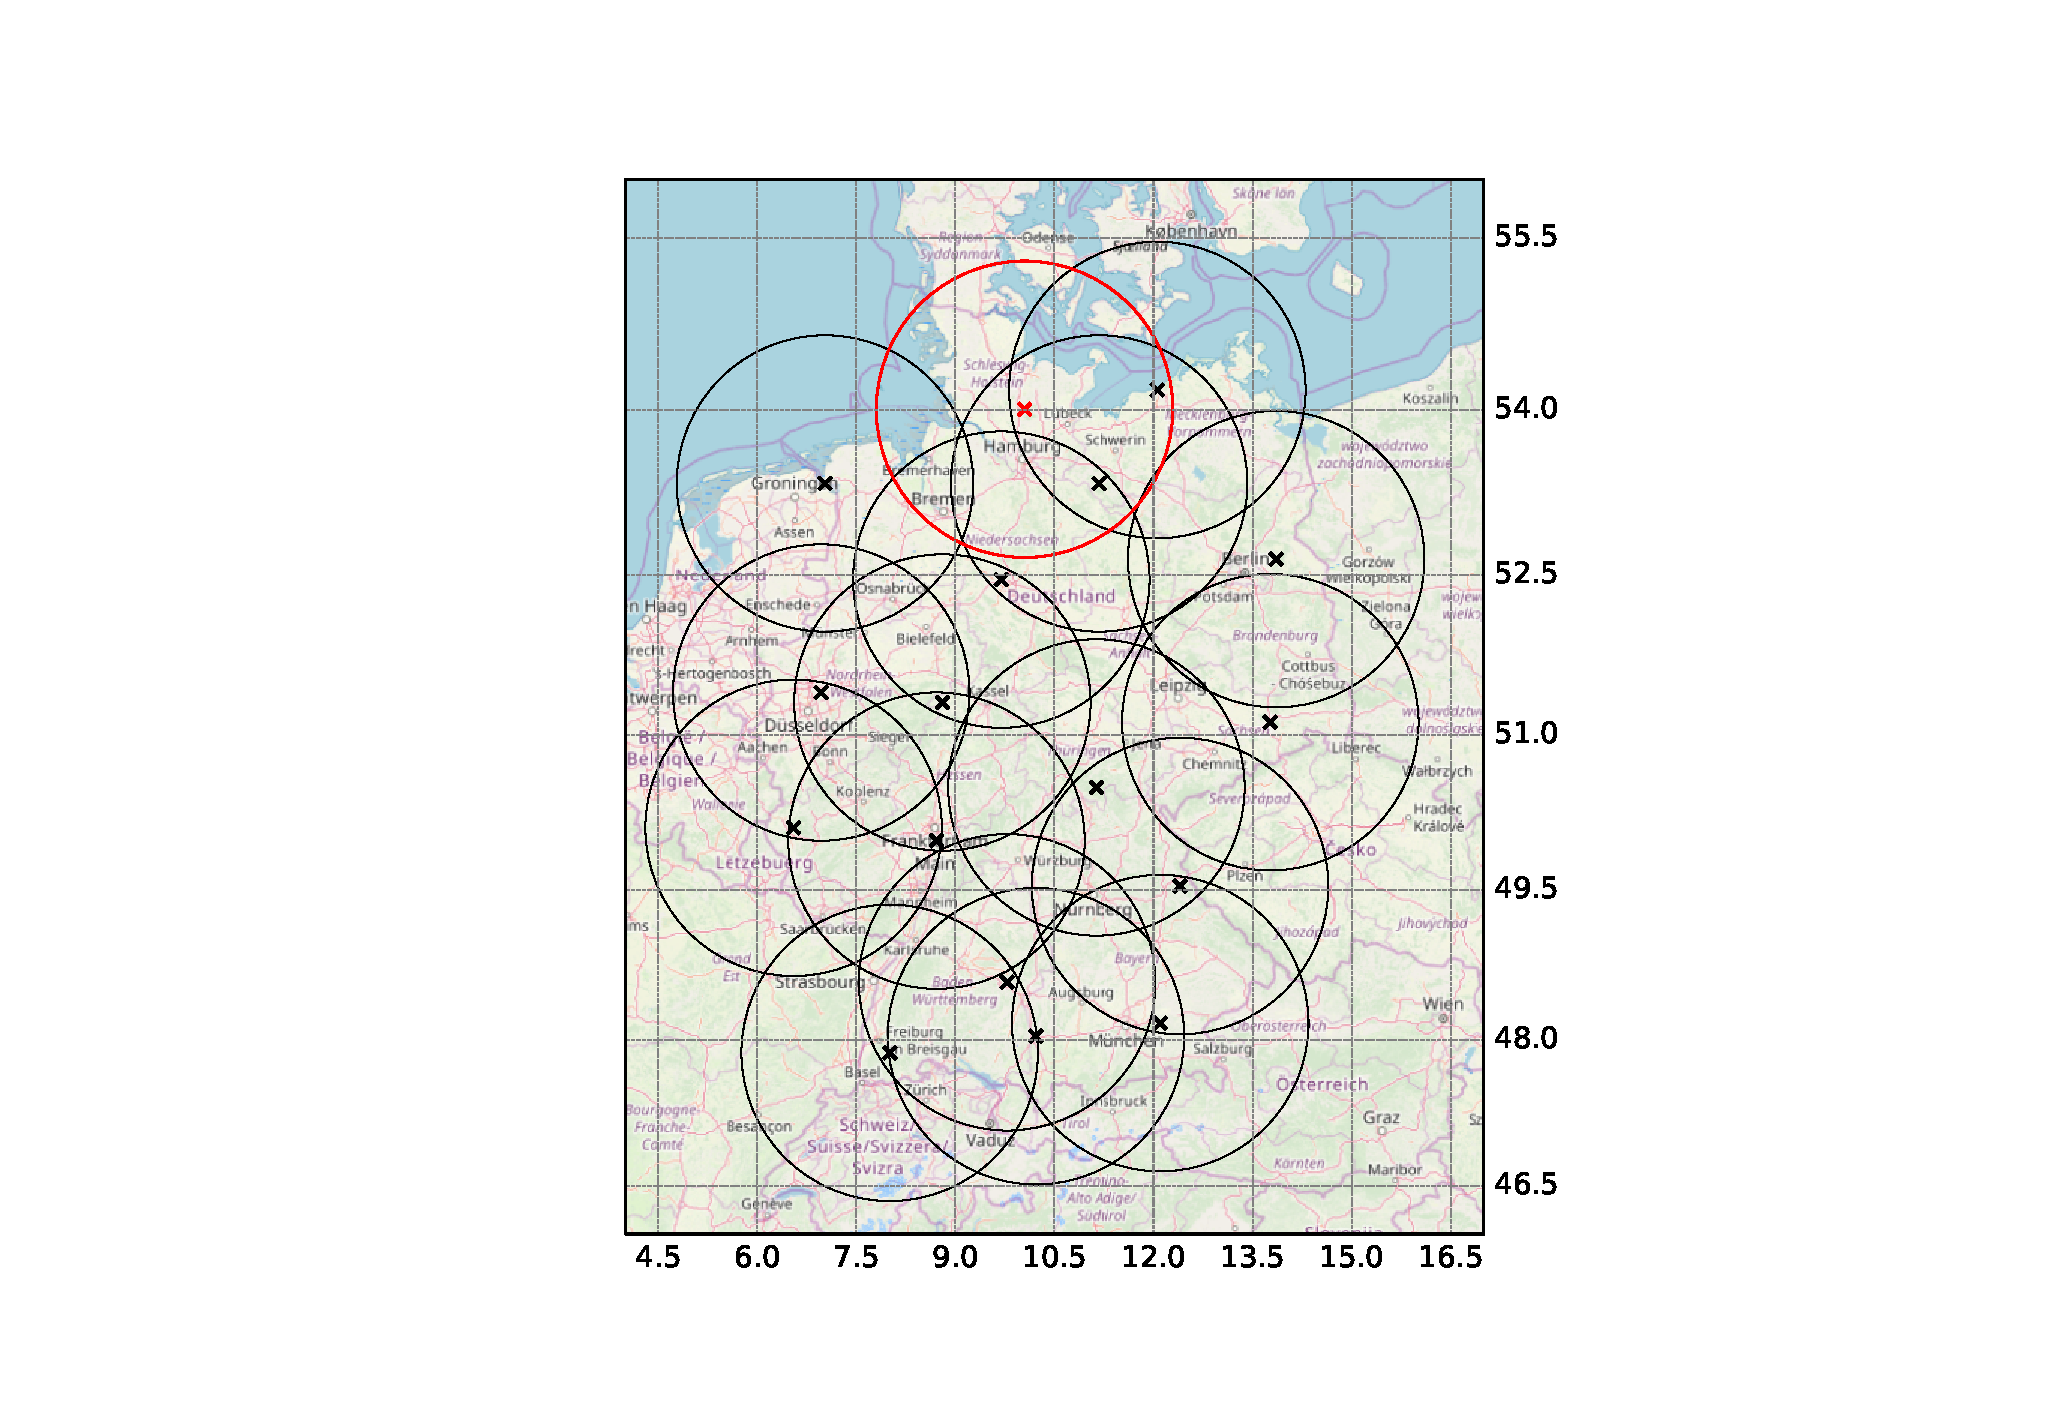
\includegraphics[width=\textwidth,trim={70mm 0 70mm 10mm}, clip]{dwdradars.eps}
	\caption[DWD radar network]{The radar network the DWD. Crosses mark the position of the operating radars. The circles show the maximum distance of the precipitation scans. The red cross and red circle show the position of the Boostedt radar and the maximum distance of the precipitation scan of the Boostedt radar.}
	\label{fig:radarnetwork}
\end{figure}


%Boostedt DWD radar site: 54.0055° N, 10.04683° E, 124.6 m height
%Precipitation scan: 0.5° ,following orographie (150 km range)
%250m range gates, 1° azimuth steps
%5 minute time resolution
%C-Band
%100 km x 100 km box around PATTERN radar position taken from the whole radar image
%DWSR/5001/SDP/CE
\FloatBarrier
\section{Hamburg Radar Data}
%TODO 
The Precipitation and Attenuation Estimates from a High-Resolution Weather Radar Network (PATTERN) project aimed to investigate low cost local area weather radars (LAWR) and if they can operate as a complement to nationwide radar networks \citep{Lengfeld2014}. One radar in the PATTERN project is set up in the city of Hamburg on top of the Geomatikum in a height of 90\,m above ground (black circle in Figure \ref{fig:radarOverview}). The location of the radar is 53.56833°\,N, 9.97997°\,E and has a distance of approx. 30\,km to the Boostedt radar. The radar operates on a frequency of 9410\,MHz and a wavelength of approx. 3.2\,µm. This classifies the radar as a X-band radar. The X-band radars in the PATTERN project are not capable of measuring in Doppler or dual-polarisation mode \citep{Lengfeld2014}.\\
The Hamburg radar data has a range resolution of 60\,m, 1° angular resolution and a temporal resolution of 30\,s. The maximum range is 20\,km. The technical specifications of the Hamburg radars are listed in Table \ref{tab:radarspec}.
% https://wetterradar.uni-hamburg.de/index.php?id=4035

\begin{table}[!htbp]
	\centering
	\caption[]{Hamburg and DWD radar specifications from \citep{Lengfeld2014} and \citep{Frech2013}.}
	\label{tab:radarspec}
	\begin{tabular}{|l|l|l|}
		\hline
		Performance parameters &DWD & Hamburg radar\\\hline
		Range resolution & 250\,m & 60\,m\\
		Time resolution & 300\,s & 30\,s\\
		Angular resolution & 1\deg & 2.8\deg\\
		Sampling resolution in azimuth & 1\deg & 1\deg\\
		Maximum range& 150\,km & 20\,km\\
		Calibration accuracy& $2$ & $\pm1$\,dB\\
		Transmit power & 500\,kW & 25\,kW\\
		Frequency & 5600-5650\,MHz & 9410\,MHz\\
		Pulse width & 0.4 or 0.8\,µs & 0.4\,µs \\
		Pulse repetition frequency & 600\,Hz & 800\,Hz  \\
		Beam width & 1\deg & 2.8\deg \\\hline
	\end{tabular}
\end{table}
\begin{figure}[!htbp]
	\centering
	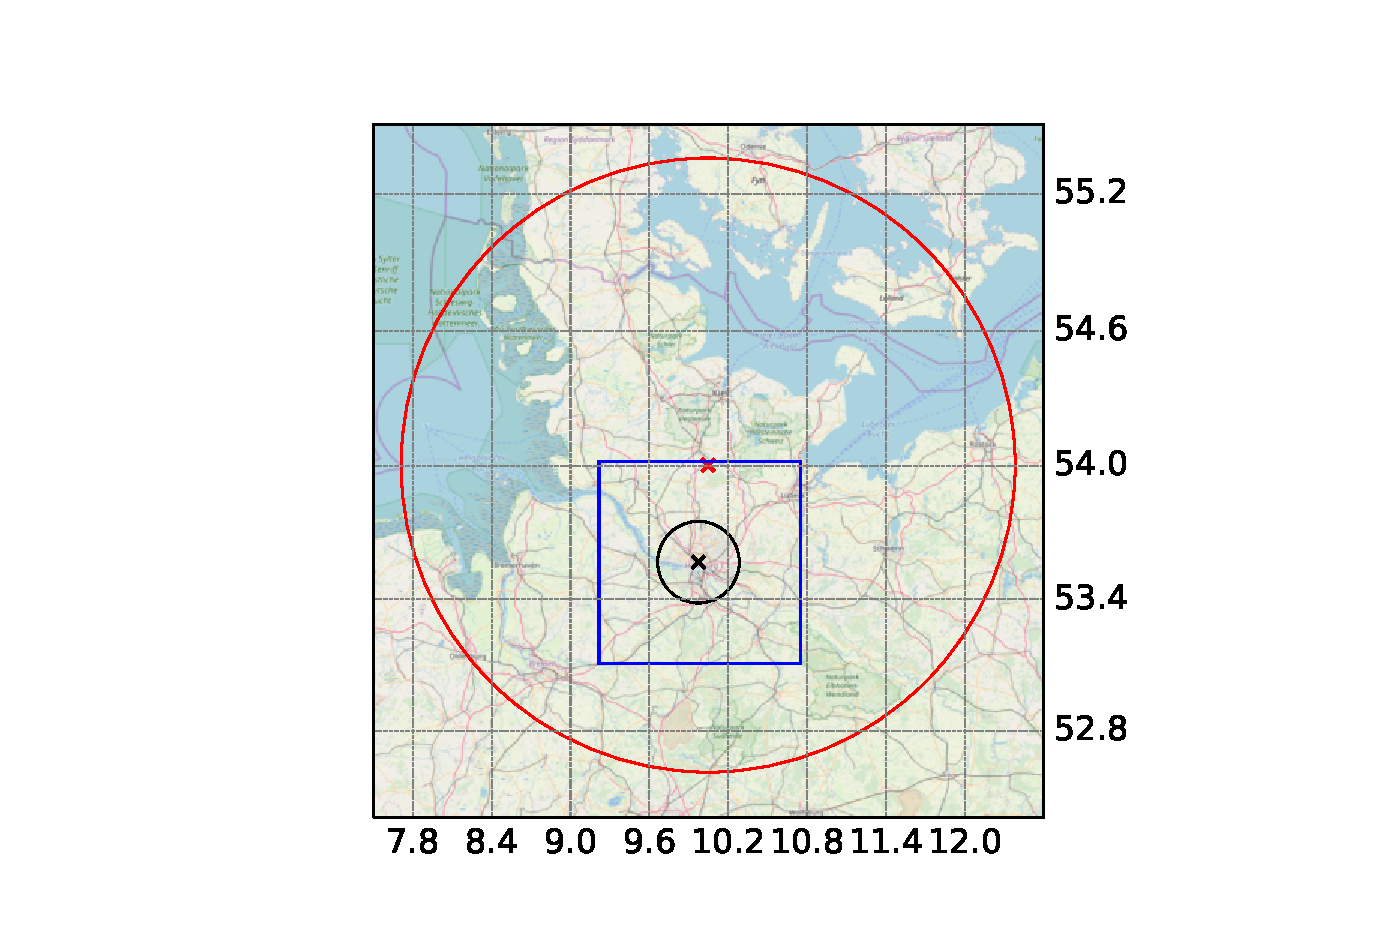
\includegraphics[width=\textwidth,trim={20mm 0 20mm 0}, clip]{radarOverview.eps}
	\caption{Radaroverview. Red: Boostedt precip sweep, Black: Pattern precip sweep, Blue: Nesting area from boostedt radar sweep}
	\label{fig:radarOverview}
\end{figure}
\chapter{Prognosis Model}
The developed prognosis model is a combination of a linear advection model and a probabilistic nowcasting model. It uses radar precipitation fields from the Boostedt and Hamburg radar to perform a short-term precipitation forecast. The prognosis is based on field based motion detection between two consecutive radar scans, motivated by identifying local maxima and their movement over time in the precipitation field.
\section{Overview}
The general workflow of the model is given in Figure \ref{fig:model}. In the following sections a more detailed description for the model and the used methods is given. Before the model can be launched, several parameters and paths to the input fields need to be set. %(section \ref{subsec:param}). 
Then the radar data for DWD and PATTERN (section \ref{chap:data}) is read. This radar data is then gridded and interpolated to their respective grids (section \ref{subsec:grid}). Now both the DWD and PATTERN radar data is on a Cartesian grid and ready for further usage. \\
First the displacement detection algorithm (section \ref{subsec:disdetect}) is applied to both the DWD and PATTERN precipitation field. The displacements of the precipitation fields of DWD and PATTERN are then evaluated separately to identify erroneous displacements. In case no valid displacements can be detected in the DWD or PATTERN precipitation fields, the results from the displacement detection from one radar is used for the other radar. If at all no valid displacements can be detected the model fails and a prognosis can not be made. \\
Now the displacement parameters from the DWD and PATTERN precipitation fields are used to perform the extrapolation for both precipitation fields (section \ref{subsec:extrapolation}). The Cartesian DWD precipitation fields are extrapolated with Lagrangian persistence \citep{Germann}. The extrapolation of the DWD precipitation fields is then used as the parent domain for the PATTERN extrapolation. \\
The nested PATTERN precipitation data is then extrapolated via Gauss filtering using the properties of a bivariate normal density distribution (section \ref{subsec:bivar}) constructed from the previously determined parameters of the displacement distribution (section \ref{subsec:disdetect}). This extrapolation is then the result for the total prognosis. With reference data the skill of the prognosis is evaluated by calculating several forecast skill scores (section \ref{subsec:eval}).
\begin{figure}[!htbp]
\centering
	\begin{tikzpicture}[%
		>=triangle 60,              % Nice arrows; your taste may be different
		start chain=going below,    % General flow is top-to-bottom
		node distance=10mm and 10mm, % Global setup of box spacing
		every join/.style={norm},   % Default linetype for connecting boxes
		]
		\tikzset{
			>={Latex[width=2mm,length=2mm]},
			base/.style={draw, on chain, on grid, align=center, minimum height=4ex},
			proc/.style={base, rectangle, text width=8em},
			test/.style={base, diamond, aspect=2, text width=5em},
			term/.style={proc, rounded corners},
			% coord node style is used for placing corners of connecting lines
			coord/.style={coordinate, on chain, on grid},
			% nmark node style is used for coordinate debugging marks
			nmark/.style={draw, cyan, circle, font={\sffamily\bfseries}},
			% -------------------------------------------------
			% Connector line styles for different parts of the diagram
			norm/.style={->, draw, lcnorm},
			free/.style={->, draw, lcfree},
			cong/.style={->, draw, lccong},
			it/.style={font={\small\itshape}}
		}
	
	\node [proc, densely dotted] (b0) {Setting of input and parameters};
	\node [term,lcnorm,left of=b0,xshift=-3cm]  (p1)    {PATTERN Input};
	\node [term,lccong,right of=b0,xshift=3cm]  (d1)    {DWD Input};
	\node [proc,densely dotted,below of=b0] (b1) {Gridding and Interpolation};
	\node [term,lcnorm,below of=b1,xshift=-2cm]  (p2)    {Cartesian data of PATTERN};
	\node [term,lccong,below of=b1,xshift=2cm]  (d2)    {Cartesian data of DWD};
	\node [proc,densely dotted,below of=b1,yshift=-2cm] (b3) {Displacement detection};
	\node [proc,densely dotted,below of=b3] (b4) {Displacement evaluation};
	\node [proc,densely dotted,below of=b4] (b5) {Exchange of parameters if necessary};
	\node [term,lcnorm,below of=b5,xshift=-2cm]  (p3)    {PATTERN displacement parameters};
	\node [term,lccong,below of=b5,xshift=2cm]  (d3)    {DWD displacement parameters};
	\node [proc,lccong,densely dotted,below of=d3] (d4) {Extrapolation of DWD via Lagrangian persistence};
	\node [term,lccong,below of=d4] (d5) {Parent domain for PATTERN};
	\node [proc,densely dotted, below of=b5,yshift=-6cm] (b6) {Extrapolation of nested PATTERN via Gauss filtering};
	\node [term, below of=b6] (b7) {Prognosis for nested PATTERN};
	\node [term, below of=b6,xshift=4cm] (b8) {Scores};
	\node [coordinate,right of=d2,xshift = 2cm] (dummy0) {};
	\node [coordinate,right of=d4,xshift = 2cm] (dummy1) {};
	\node [coordinate,left of=p2,xshift = -2cm] (pummy0) {};
	\node [coordinate,left of=b6,xshift = -4cm] (pummy1) {};
	\path[->, to path={-| (\tikztotarget)}] (b0) edge (p1);
	\path[->, to path={-| (\tikztotarget)}] (b0) edge (d1);
	\path[->, to path={|- (\tikztotarget)}] (p1) edge (b1);
	\path[->, to path={|- (\tikztotarget)}] (d1) edge (b1);
	\draw[->] (b1)--(p2);
	\draw[->] (b1)--(d2);
	\draw[->] (p2)--(b3);
	\draw[->] (d2)--(b3);
	\draw[->] (b3)--(b4);
	\draw[->] (b4)--(b5);
	\draw[->] (b5)--(p3);
	\draw[->] (b5)--(d3);
	\draw[->] (d3)--(d4);
	\draw[->] (d3)--(d4);
	\draw[->] (d4)--(d5);
	\path[->, to path={-| (\tikztotarget)}] (d5) edge (b6);
	\path[->, to path={-| (\tikztotarget)}] (p3) edge (b6);
	\draw[->] (b6)--(b7);
	\draw[->] (b7)--(b8);

	%\path[->, to path={|- (\tikztotarget)}] (d2) edge (d4);
	\draw[->] (d2)--(dummy0)--(dummy1)--(d4);
	\draw[->] (p2)--(pummy0)--(pummy1)--(b6);
	\end{tikzpicture}
	\caption[Modelflowchart]{Flowchart for the model structure. Rectangular boxes show methods and algorithms. Rounded boxes show data output. Red coloured boxes show methods, algorithms and data output for the DWD data. Blue respectively for PATTERN. Black coloured boxes are used for methods, algorithm and data output which involve data from both DWD and PATTERN.}
	\label{fig:model}
\end{figure}

\section{Gridding and Coordinate Transformation}
\label{subsec:grid}
The DWD and PATTERN radar data is available as radar reflectivity. Reflectivity $z$ is a measure for the energy intensity which is backscattered by remote objects. The reflectivity $z$ is given in [mm$^{6}$m$^{-3}$] and is proportional to the number of droplets and the size of the droplets. The reflectivity is more often used in its logarithmic form $Z$ in [dBZ] and is calculated from $z$ with eq. \ref{eq:dBZ}. The logarithmic form of the reflectivity is mostly used to make it more readable.
\begin{equation}
Z  = 10 \cdot \log _{10}(z)
\label{eq:dBZ}
\end{equation}
From the reflectivity $z$ the precipitation rate $R$ in [mmh$^{-1}$] can be derived via a common empirical z-R-relation:
\begin{equation}
z = aR^{b},
\label{eq:zr}
\end{equation}
where a and b are empirically-derived parameters. DWD and PATTERN use following values for the z-r-relation for different radar reflectivities \citep{Lengfeld2014}:

%\begin{equation}
%	R = \frac{z}{a}^{\frac{1}{b}}
%\end{equation}

\begin{equation}
\begin{array}{lcl}
Z \le 36.5 \text{dBZ}: & a = 320, b = 1.4 \\
36.5 \text{dBZ} < Z \le 44.0 \text{dBZ}: & a  = 200, b = 1.6 \\
Z > 44.0 \text{dBZ}: & a = 77, b = 1.9
\end{array}
\end{equation}
Initially both the DWD and PATTERN radar data are on a polar grid around their respective radar stations. For simpler grid operations and easier comparability the polar radar data of DWD and PATTERN is transformed and gridded to Cartesian grids. To perform a coordinate transformation from a spheroid to a plane a sophisticated map projection is needed. This is done by using the Transverse Mercator projection, which transforms the polar grid coordinates to Cartesian grid coordinates. For the nesting of the radars the map projection needs to have a high accuracy with regard to earth's curvature. The Transverse Mercator projection is a very accurate map projection \citep{Karney2011}, which divides the Earth into 60 zones with 6° longitude in width \citep{TMP}. Hamburg and its surrounding area lies in the EPSG zone number 32632.\\ %(Fig. \ref{fig:EPSG}).\\%Displacing the point of origin in the coordinate system from the point of the radar to the EPSG zone 32632.
The polar coordinates of the radar data are defined by the azimuth angle $azi$ and distance from the radar $r$. With eq. \ref{eq:trans} the polar coordinates are transformed to Cartesian distances to the radar.
%\begin{figure}[!htbp]
%	\centering
%	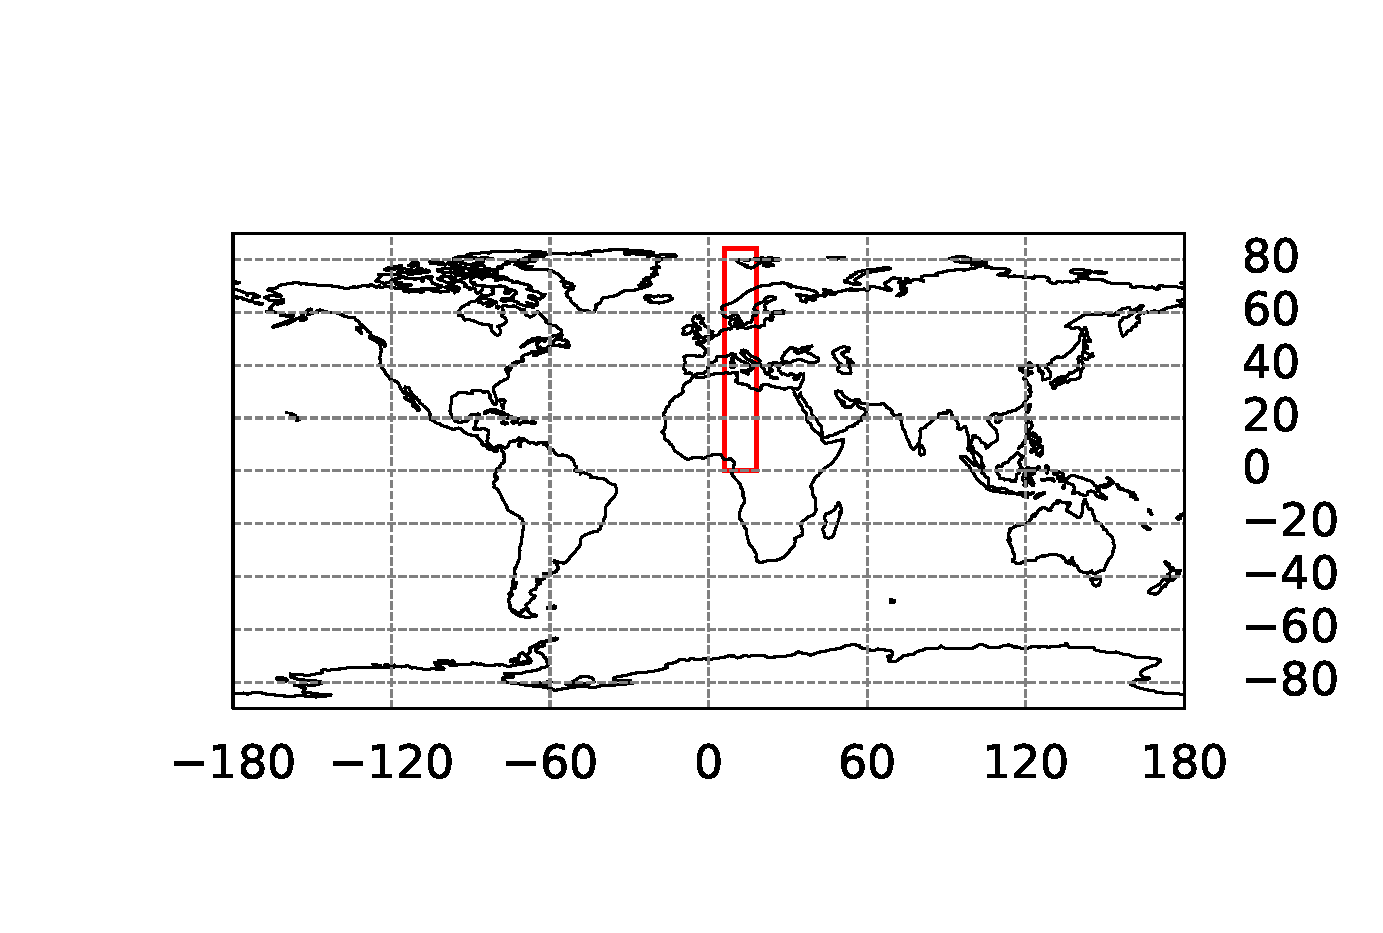
\includegraphics[width=\textwidth]{EPSG2.eps}
%	\caption{Overview of the EPSG zone number 32632.}
%	\label{fig:EPSG}
%\end{figure}
\begin{equation}
	\begin{array}{lcl}
		x = r \cdot \cos(azi)\\
		y = r \cdot \sin(azi)
	\end{array}	
	\label{eq:trans}
\end{equation}%%This immensely reduces the computational work, but still lengthens the possible lead time for a precipitation forecast for Hamburg. \\ % hier vielleicht noch was über verlängerung der prognosezeit. %Hier noch den typ der daten, CLT corrected,xband,cband
The Cartesian distances to the radar are then transformed to Cartesian coordinates with the Transverse Mercator projection \footnote{For the Transverse Mercator projection the 'Geospatial Data Abstraction Library' (GDAL) and the python module 'osgeo' is used \citep{Warmerdam}. Documentation for GDAL: 'gdal.org/python'.}. This is done for the coordinates of the DWD and PATTERN radars. From the DWD radar only a square with an edge length of 100\,km with the centre at the position of the PATTERN radar is used (Fig. \ref{fig:radarOverview}). Now the Cartesian coordinates for every polar grid point for the DWD and PATTERN radars are known. 
\subsection{Interpolation Methods}
\subsubsection{Barycentric Interpolation}
To transform the data from a polar grid to a Cartesian grid a Barycentric interpolation is applied to the radar data. The Barycentric interpolation is implemented following \cite{bary}. \\
For the two dimensional barycentric interpolation the first step is to arrange the initial grid, here a polar grid around the radar site, into triangles. For this the Delaunay Triangulation after \cite{delaunay} is used. This triangulation triangulates a set of points \textbf{P} so that no point in \textbf{P} is inside of the circumcircle of any triangle. Now the surrounding triangle is known for each point of the Cartesian grid.\\
In comparison to coordinate systems like Cartesian or polar coordinate systems where points are offsets to a origin, barycentric coordinates describe the position of points relative to a simplex (e.g. a point, a line, a triangle or a tetrahedron) (\citealp{bary} and \citealp{baryBerrut}). In this case barycentric coordinates are used to compare positions of points to triangles. For triangles barycentric coordinates can be understood as area coordinates. The equations to calculate the barycentric coordinates $d,e,g$ of the point $P$ in the triangle $A,B,C$ are ratios of their respective triangles and the total triangle (Fig. \ref{fig:bary}). For example the barycentric coordinate $g$ is calculated by dividing the area of the triangle $CAP$ by the area of the triangle $ABC$ (eq. \ref{eq:barycor}).

Now to get the value $f(x_p,y_p)$, the values of the points $A,B,C$ are weighted by their respective coordinate $d,e,g$ and summed up (eq. \ref{eq:baryeq}).
\begin{figure}[!htbp]
	\centering
	\begin{tikzpicture}
	
	\draw (0,0) -- (2,4) -- (4,0) -- (0,0);
	\fill (1.5,1.5) circle[radius=2pt];
	\fill (0,0) circle[radius=2pt];
	\fill (2,4) circle[radius=2pt];	
	\fill (4,0) circle[radius=2pt];	
	\draw (0,0) -- (1.5,1.5);
	\draw (2,4) -- (1.5,1.5);
	\draw (4,0) -- (1.5,1.5);
	
%	\draw (-0.3,-0.3) node {$(x_1,y_1)$};
%	\draw (4.3,-0.3) node {$(x_2,y_2)$};
%	\draw (2,4.3) node {$(x_3,y_3)$};
%	\draw (1.6,1) node {$(x,y)$};
	\draw (-0.3,-0.3) node {$A$};
	\draw (4.3,-0.3) node {$B$};
	\draw (2,4.3) node {$C$};
	\draw (1.8,1.7) node {$P$};
	
	\draw (1.6,0.5) node {$d$};
	\draw (2.4,1.8) node {$e$};
	\draw (1.2,1.8) node {$g$};
				
	\end{tikzpicture}
	\caption{Barycentric interpolation for a point $P$ in a triangle. $A$, $B$ and $C$ are data points of the surrounding triangle. $d$, $e$ and $g$ are the barycentric coordinates of the point $P$.}
	\label{fig:bary}
\end{figure}


\begin{equation}
	\begin{aligned}
		d = \dfrac{\Delta ABP}{\Delta ABC}\\
		e = \dfrac{\Delta BCP}{\Delta ABC}\\
		g = \dfrac{\Delta CAP}{\Delta ABC}
	\end{aligned}
	\label{eq:barycor}
\end{equation}

\begin{equation}
f(x_P,y_P) = d\,f(x_A,y_A)+e\,f(x_B,y_B)+g\,f(x_C,y_C)
\label{eq:baryeq}
\end{equation}

\subsubsection{Bilinear Interpolation}
\label{subsec:binterp}
Following a similar approach as \cite{bilinear} the bilinear interpolation is implemented with eq. \ref{eq:bilinear}. The bilinear interpolation is used for data points which lie inside of a square Cartesian grid. This is depicted in Fig. \ref{fig:bilinear}. The point $(x,y)$ is surrounded by the points $(x_1,y_1),(x_2,y_1),(x_2,y_2),(x_1,y_2)$. Now to calculate the value $f(x,y)$, the values of the surrounding points $f(x_1,y_1),f(x_2,y_1),f(x_2,y_2),f(x_1,y_2)$ are weighted with their respective opposite areas $m,n,o$ and $p$ and are summed up. 
\begin{figure}[!htbp]
	\centering
	\begin{tikzpicture}
	\draw (0,0) rectangle (4,4);
	\draw (0,0) rectangle (1,1);
	\draw (1,1) rectangle (4,4);
	\fill (0,0) circle[radius=2pt];
	\fill (0,4) circle[radius=2pt];
	\fill (4,0) circle[radius=2pt];
	\fill (4,4) circle[radius=2pt];
	\fill (1,1) circle[radius=2pt];
	\draw (-0.3,-0.3) node {$(x_1,y_1)$};
	\draw (-0.3,4.3) node {$(x_1,y_2)$};
	\draw (4.3,-0.3) node {$(x_2,y_1)$};
	\draw (4.3,4.3) node {$(x_2,y_2)$};
	\draw (1.5,1.3) node {$(x,y)$};
	\draw (2.5,2.5) node {$m$};
	\draw (0.5,2.5) node {$n$};
	\draw (0.5,0.5) node {$o$};
	\draw (2.5,0.5) node {$p$};
	\end{tikzpicture}
	\caption{Bilinear interpolation for a point at the coordinates $(x,y)$. The values of the data points $(x_1,y_1)$, $(x_2,y_1)$, $(x_2,y_2)$ and $(x_1,y_2)$ are weighted with their respective areas $m, n, o$ and $p$ and summed up to calculate the value for the point at the coordinates $(x,y)$.}
	\label{fig:bilinear}	
\end{figure}

\begin{equation}
	f(x,y) = m\,f(x_1,y_1)+n\,f(x_2,y_1)+o\,f(x_2,y_2)+p\,f(x_1,y_2)
	\label{eq:bilinear}
\end{equation}
\section{Displacement Detection}
\label{subsec:disdetect}
In order to detect movement in radar data at least two consecutive radar images are needed. By comparing the radar images, differences between the radar images become visible and can be used to estimate the movement between the radar images. The procedure to estimate the displacements of the precipitation fields from the differences between the radar images is described in the following sections. The general procedure for the DWD and PATTERN radar is:
%In order to make a prognosis on the movement of precipitation fields a displacement vector is needed and several approximations are necessary. 
\begin{enumerate}
	\item Detection of suitable patches in the precipitation field for tracking (Fig. \ref{fig:maximaOverview} and Fig. \ref{fig:maximaOverviewZoom}).
	\item Tracking of the patches (Fig. \ref{fig:displacement_t0} and Fig. \ref{fig:displacement_t1}) over the evolution of several timesteps.
	\item If patches move out of the frame or tracking becomes undesirable new patches are searched in the current time step.
	\item Tracks of each individual patch are evaluated.
\end{enumerate}

%TODO blabla zu dem unterschied von dem tracking zu feldbasiert und zellbasiert
\subsection{Detection of suitable patches}
\label{subsec:detection}
To detect the displacement of the precipitation fields in the radar scans, suitable patches for tracking are needed. Selecting suitable patches is important for future tracking. Ideally the precipitation field inside each patch should remain Lagrangian persistent in the tracking time. Furthermore the precipitation field inside the patch should ideally have a distinguishable pattern so the tracking by measuring the squared Euclidean distance becomes more reliable (Fig. \ref{fig:displacement_t0} and \ref{fig:displacement_t1}). 
\begin{figure}[!htbp]
	\centering
	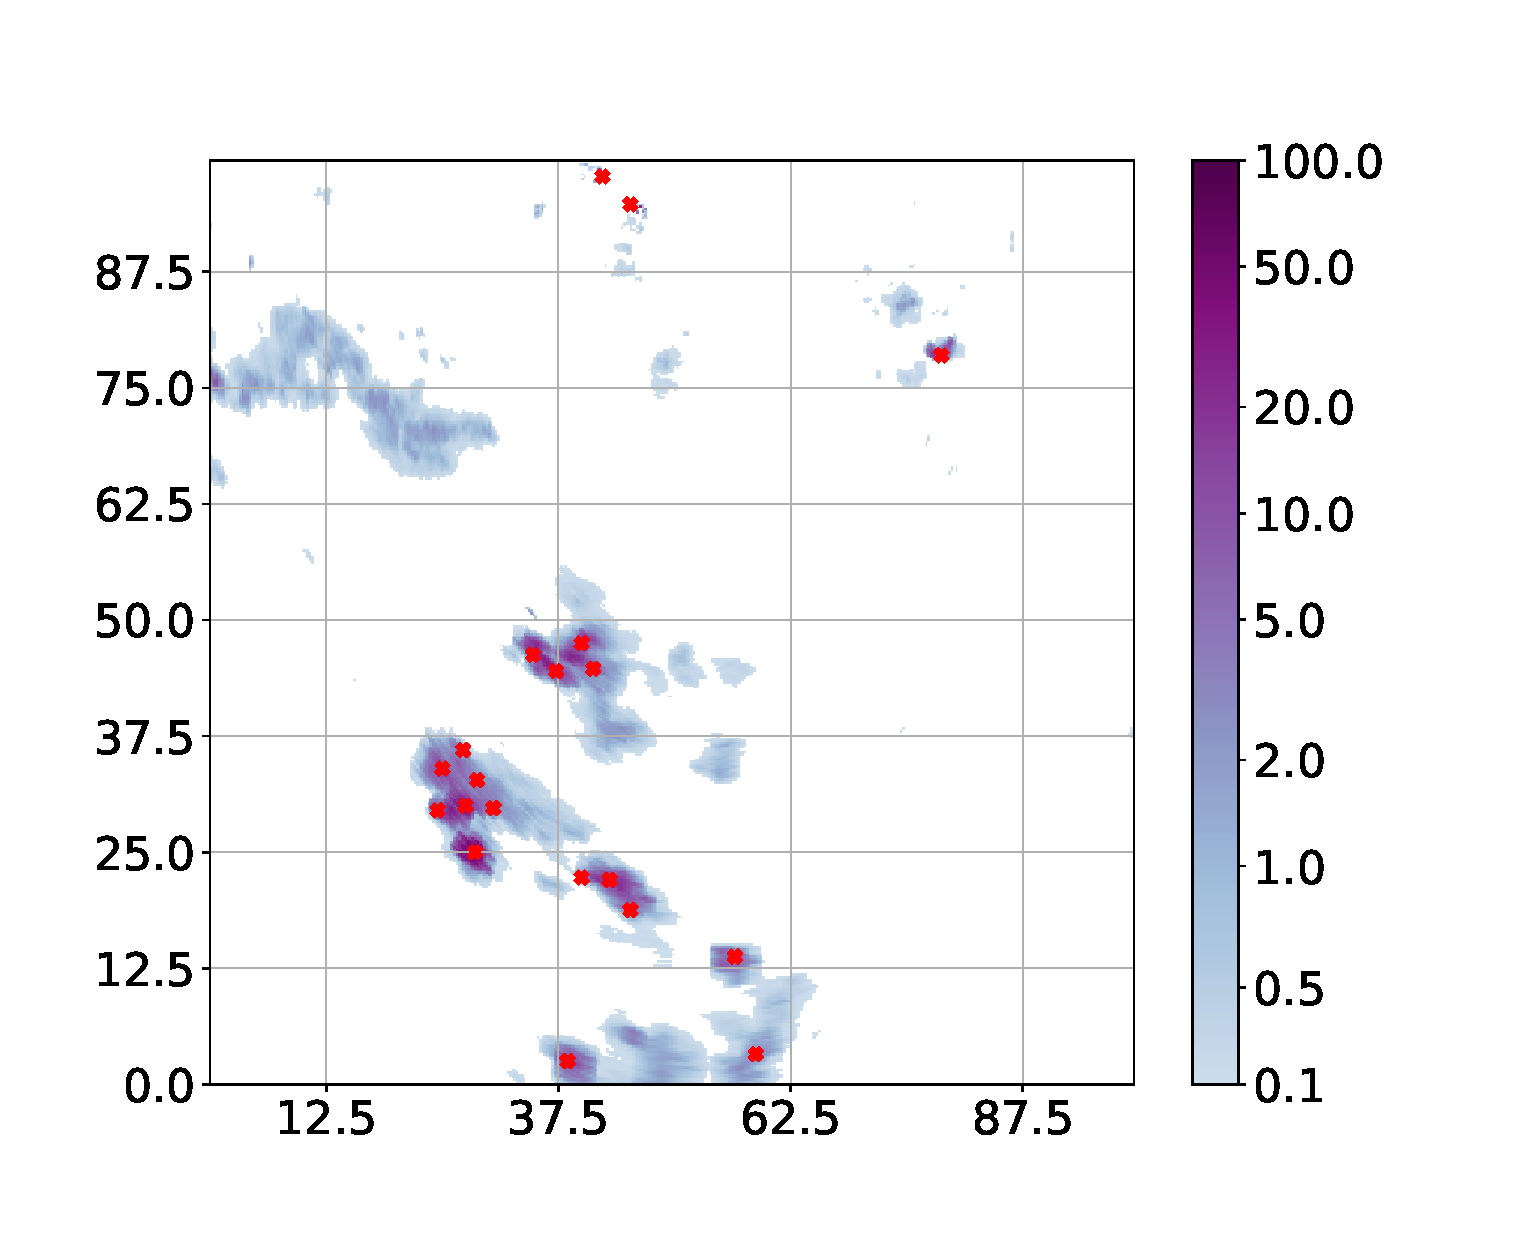
\includegraphics[width=0.9\textwidth]{maximaOverview.eps}
	\caption{Section of the DWD radar precipitation scan, with local maxima marked with a red 'x'. Precipitation scan from the 13th June 2016, 19:20 UTC.}
	\label{fig:maximaOverview}
\end{figure}
The patches are then iteratively selected by the following procedure. First the pixel with the highest rain rate inside the precipitation field is chosen. That pixel is then set as the middle point of the first patch. The patch is a square with a edge length of 2\,km for the PATTERN radar and a 12\,km for the DWD radar. The next patch is then located around the pixel with the second highest rain rate inside the precipitation field. The centre of the next patch also needs to have a minimum distance of 3\,km to the centre of the first patch to reduce the overlap of the patches (Fig. \ref{fig:maximaOverviewZoom}). The location of the third patch is then centred around the pixel with next highest rain rate, again with a minimum distance of 3\,km to any other centre. This procedure is then continued until a specific number of patches are chosen or no more pixels with a minimum rain rate of over 0.5\,mm and a minimum distance of 3\,km to all other centres can be found inside the radar image.
\subsection{Tracking of the patches}
To get information about the displacement of the precipitation fields the position of the patches in the radar scans is tracked for 8 minutes for the PATTERN radar and 25 minutes for the DWD radar. This is done by estimating the displacement of each patch between two timesteps by calculating the squared euclidean distance (Fig \ref{fig:displacement_t0} and \ref{fig:displacement_t1}). To estimate the displacement of one patch the patch in the radar image at the time $t$ (Fig. \ref{fig:displacement_t0}) is 'searched' in the radar image of the next time step $t + 1$ (Fig. \ref{fig:displacement_t1}). The search area is a square with double the edge length of a patch, 4\,km for the PATTERN radar and 24\,km for the DWD radar. Then the squared euclidean distance is calculated between the patch and the total area of the 'search' area. The squared Euclidean distance is calculated with eq. \ref{eq:crosscorr} after \cite{crosscorr}. 
\begin{figure}[!htbp]
	\centering
	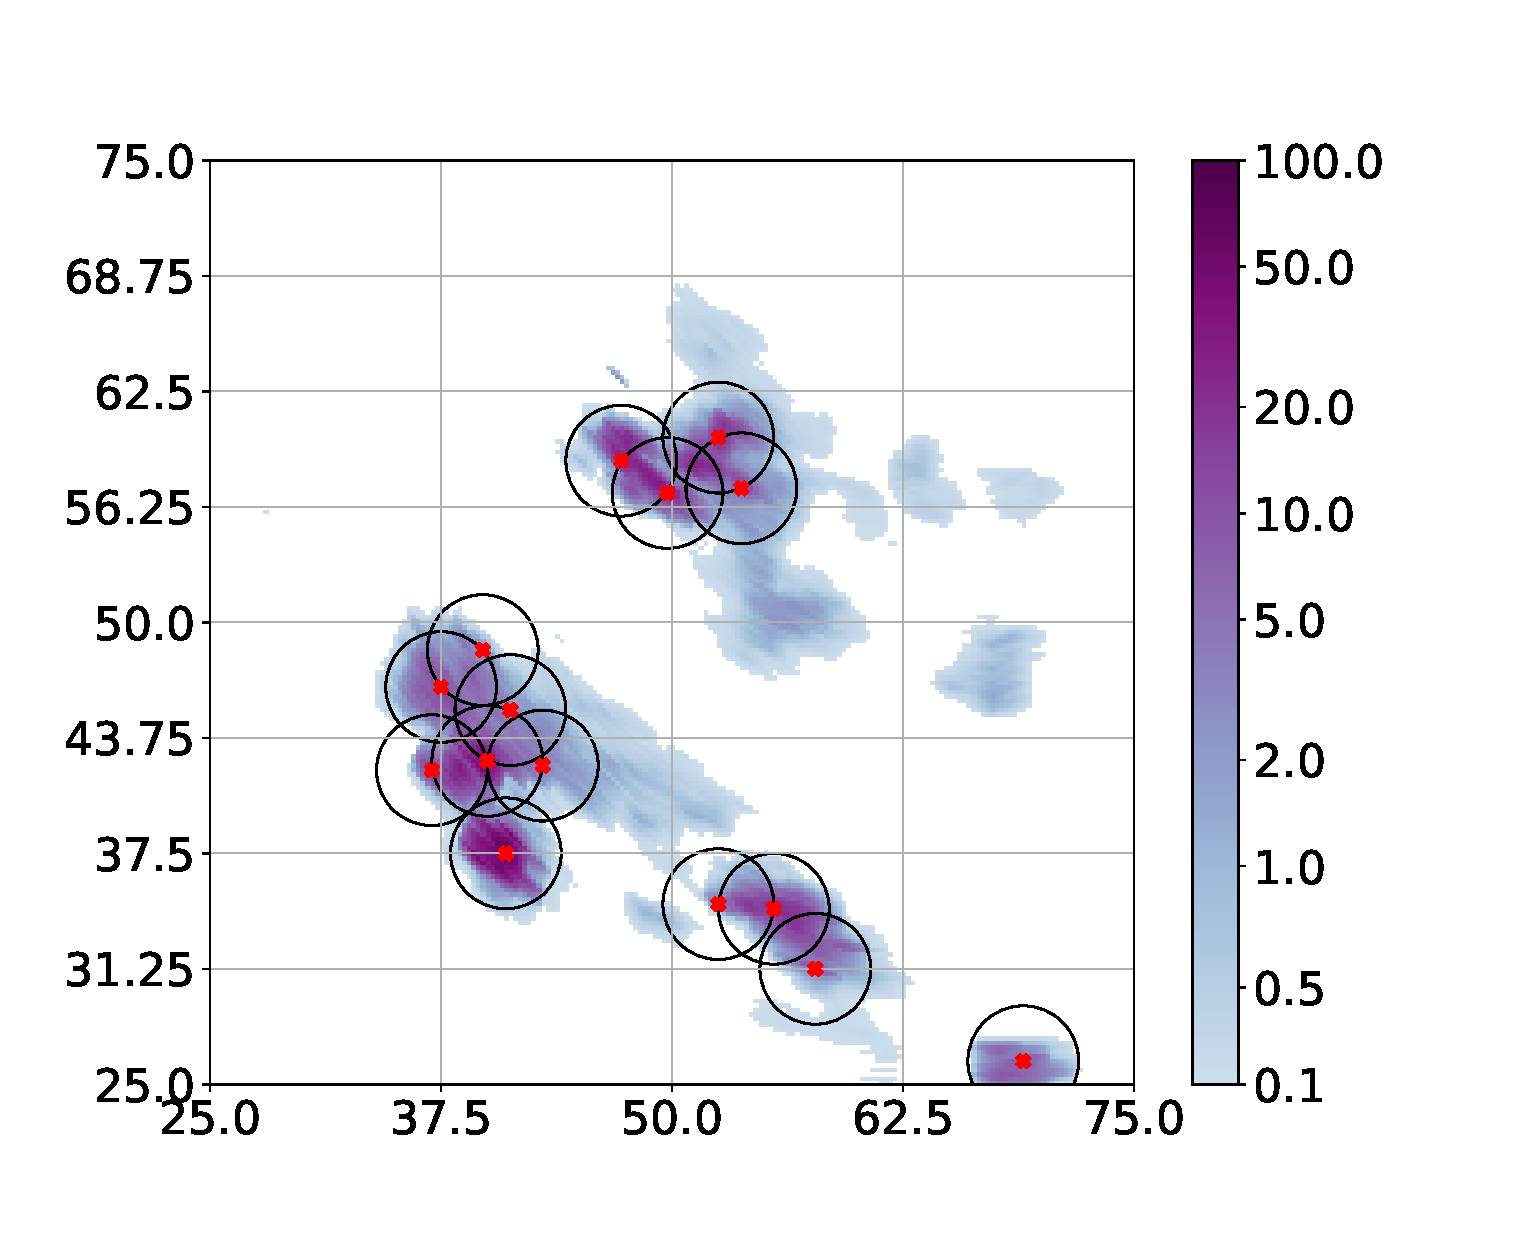
\includegraphics[width=0.9\textwidth]{maximaOverviewZoom.eps}
	\caption{Section of the DWD radar precipitation scan, with the maxima marked with 'x', and black circles for showing the minimum distance between the local maxima. Precipitation scan of the DWD radar at the 13th June 2016, 19:20 UTC.}
	\label{fig:maximaOverviewZoom}
\end{figure}
%TODO hier noch ne abbildung mit nem suchquadrat in die abbildung displacement_t1
%http://www.cs.umd.edu/~djacobs/CMSC426/Convolution.pdf
\begin{equation}
d^2_{q,p}(u,v) = \sum_{x,y}^{}\big[q(x,y)-p(x-u,y-v)\big]^2
\label{eq:crosscorr}
\end{equation}
In eq. \ref{eq:crosscorr} $q$ is the patch and $p$ is the 'search' area. The sum is over $x$, $y$ of the window of the 'search area' $p$ positioned at $u$, $v$.\\
By calculating the squared Euclidean distance for every possible position of the patch over the 'search' area, you get a matrix of squared Euclidean distances for all possible positions (Fig. \ref{fig:corr_matrix}). Small values indicate a small squared Euclidean distance and high values a high squared Euclidean distance. A small squared Euclidean distance indicates a high similarity between the patch and the corresponding window used for the calculation of the squared Euclidean distance and a high squared Euclidean distance vice versa a low similarity. The absolute values of the squared Euclidean distance are not of interest here, so a normalization is not necessary. \\
The lowest squared Euclidean distance here is indicated by the black cross. The original position of the centre of the patch is indicated by the white cross. Thus the estimated displacement of the patch over one time step is the offset between the white and black cross.\\
This procedure is then applied over the total time and all patches. If the centre of a patch moves out of the radar frame or the total number of pixels inside a patch with a rain rate above 0.5\,mmh$ ^{-1}$ falls below 20, then the patch is discarded and a new patch is selected by the procedure described in section \ref{subsec:detection}. 
\begin{figure}[!htbp]
	\centering
	\begin{minipage}{0.48\textwidth}
		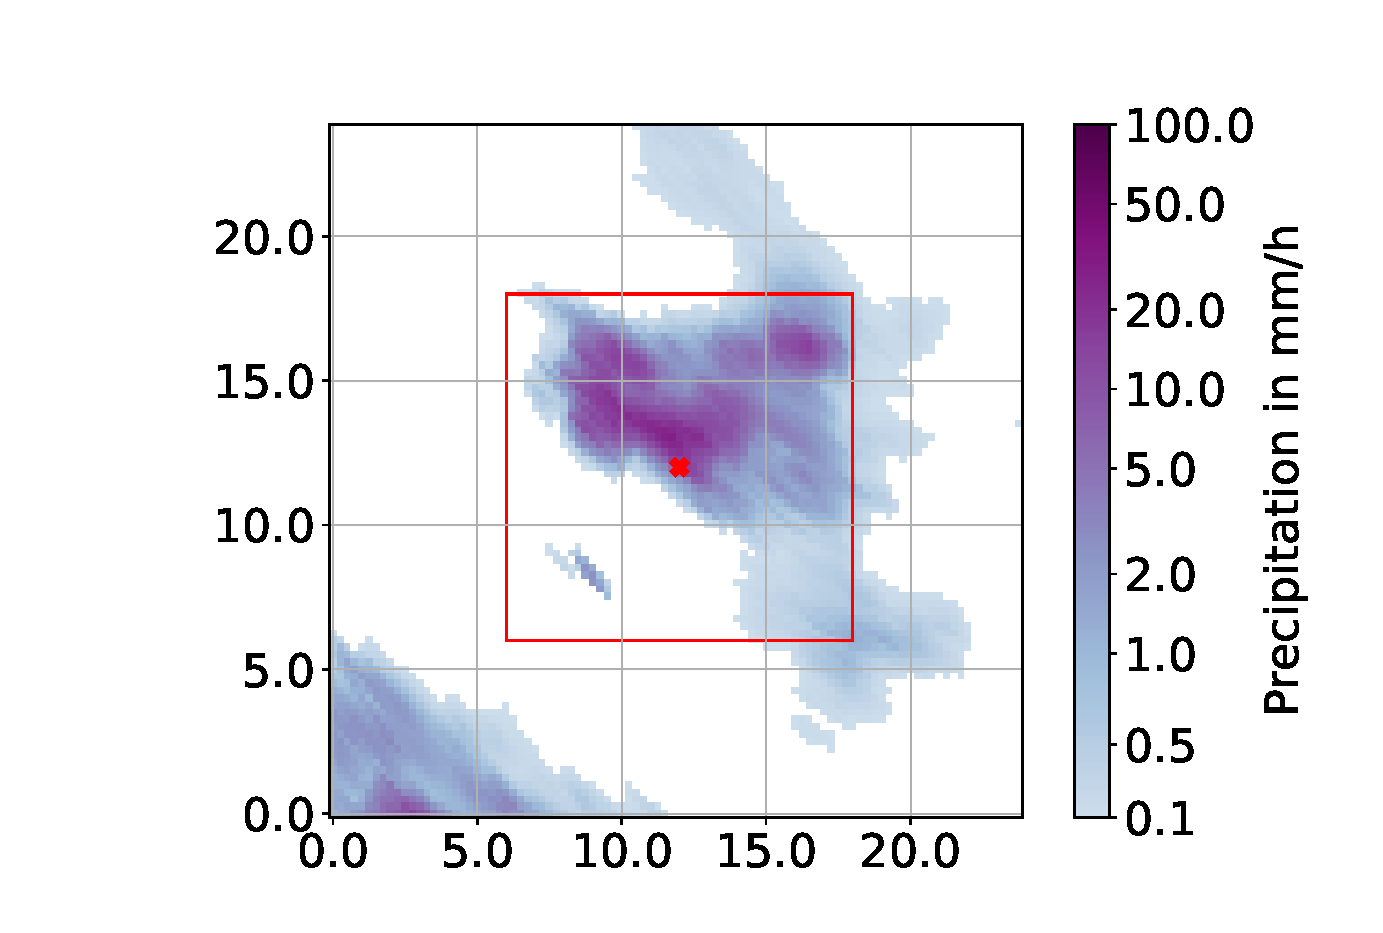
\includegraphics[width=\textwidth,trim={32mm 0 5mm 0},clip]{displacement_t0.eps}
		\caption{Section of the DWD radar precipitation scan at timestep $t=0$ at the 13th June 2016, 19:20 UTC.}
		\label{fig:displacement_t0}
	\end{minipage}\hfill
	\begin{minipage}{0.48\textwidth}
		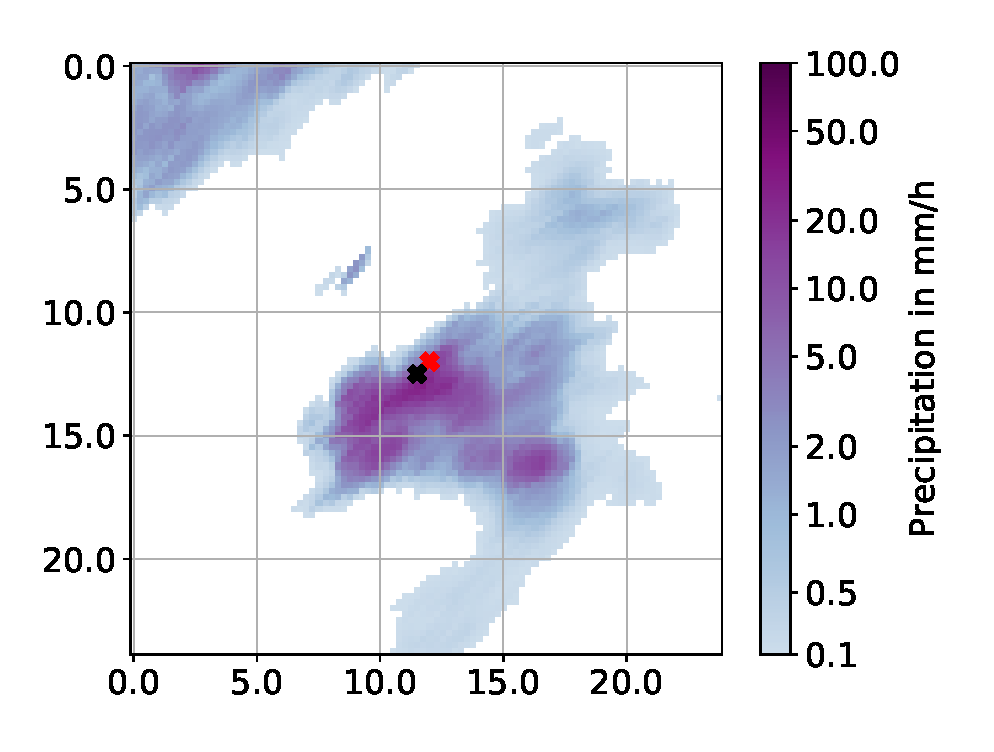
\includegraphics[width=\textwidth,trim={32mm 0 5mm 0},clip]{displacement_t1.eps}
		\caption{Section of the DWD radar precipitation scan at timestep $t=1$ at the 13th June 2016, 19:25 UTC.}
		\label{fig:displacement_t1}
	\end{minipage}
\end{figure}

\begin{figure}[!htbp]
	\centering
	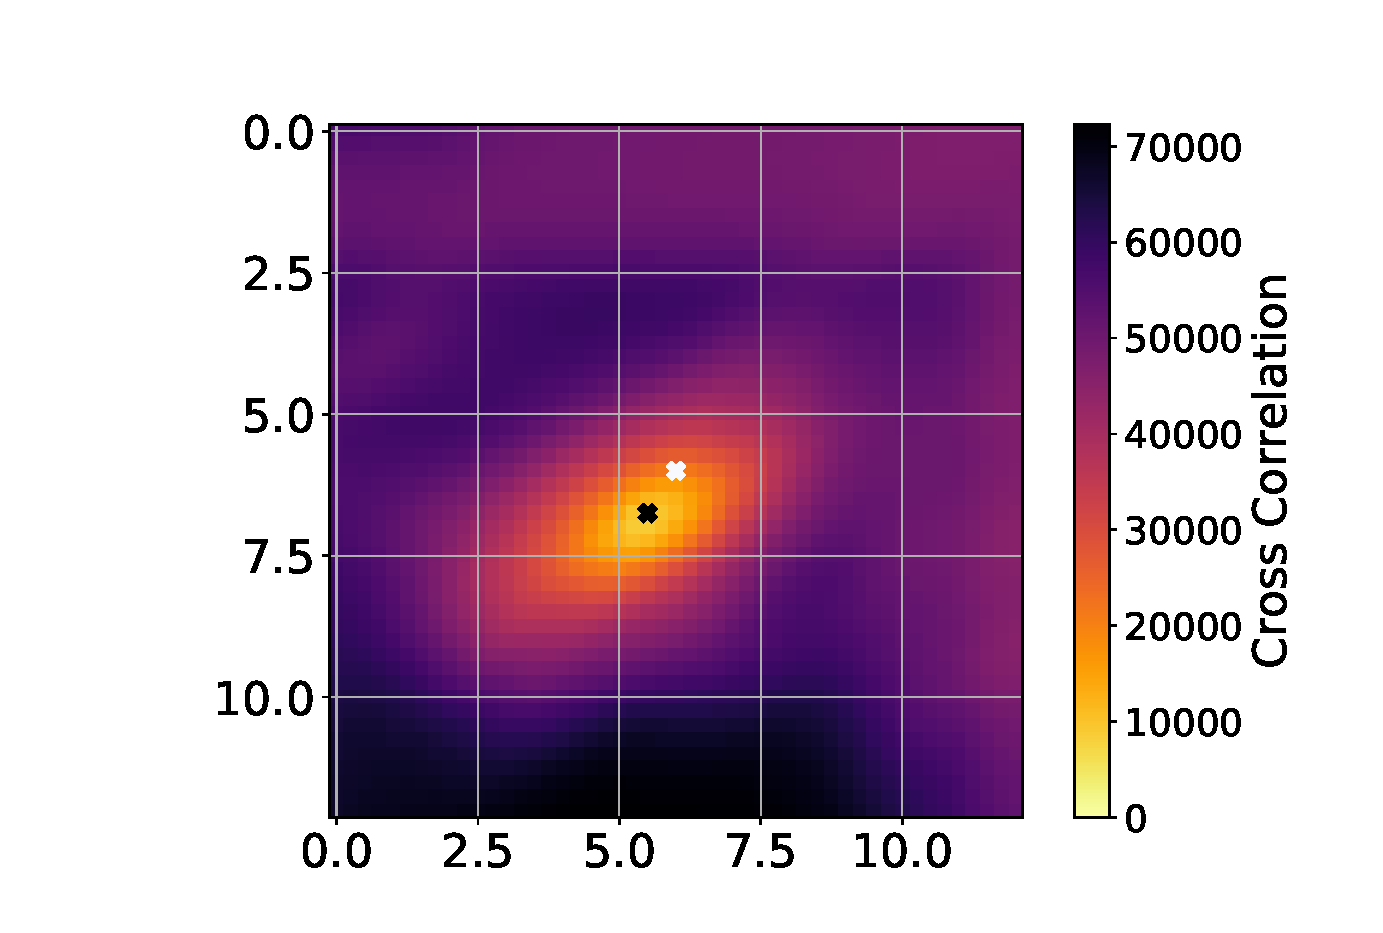
\includegraphics[width=0.9\textwidth,trim={5mm 0 5mm 0},clip]{Correlation_Matrix.eps}
	\caption{Squared euclidean distance matrix between the red square from Fig. \ref{fig:displacement_t0} at timestep $t=0$ and the total area of Fig. \ref{fig:displacement_t1} at timestep $t=1$. The white $x$ marks the centre of the matrix. The black $x$ marks the minimum value of the squared euclidean distance. The offset between the white $x$ and the black $x$ is the estimated displacement of the red square from Fig. \ref{fig:displacement_t0} at timestep $t=0$ to the total area of Fig. \ref{fig:displacement_t1} at timestep $t=1$.}
	\label{fig:corr_matrix}
\end{figure}

\subsection{Evaluation of the tracks}
After estimating the displacements for all patches over the specified time periods, the tracks (multiple displacements) need to be checked for errors. The estimation of the displacements is due to various reasons not perfect. Changes in the precipitation field like a strengthening or weakening rain rate can cause a wrong displacement detection. Furthermore, possible in case of stratiform precipitation, a very uniform precipitation pattern in the patch and in the 'search' area can lead to an erroneous displacement detection.\\
To differentiate good from bad tracks an orthogonal distance regression (ODR) (Fig. \ref{fig:orthogonaldist}) for each track (Fig. \ref{fig:displacement}) is performed. The ODR calculates a line through a dataset of points which minimizes the squared distances from the points to their foot points on the line. \\
The squared distance of all points to their respective foot points on line (red lines in Fig. \ref{fig:orthogonaldist}) is then summed up. If this sum is bigger than the halved distance between the first and last point (dotted line) the track is rejected. The example track in Fig \ref{fig:orthogonaldist} would be rejected. \\
From all accepted tracks a mean displacement in $x$ and $y$ direction is now calculated. Additionally the covariances between all displacements, $x$ and $x$,  $x$ and $y$, $y$ and $x$ and $y$ and $y$ are calculated to know how the displacements vary with each other. These parameters are calculated for the tracks of the DWD and the PATTERN precipitation fields. 
If no acceptable displacements can be found for either one of the precipitation fields, the displacements from one of the precipitation fields are used for the other precipitation field.

\begin{figure}[!htbp]
	\centering
	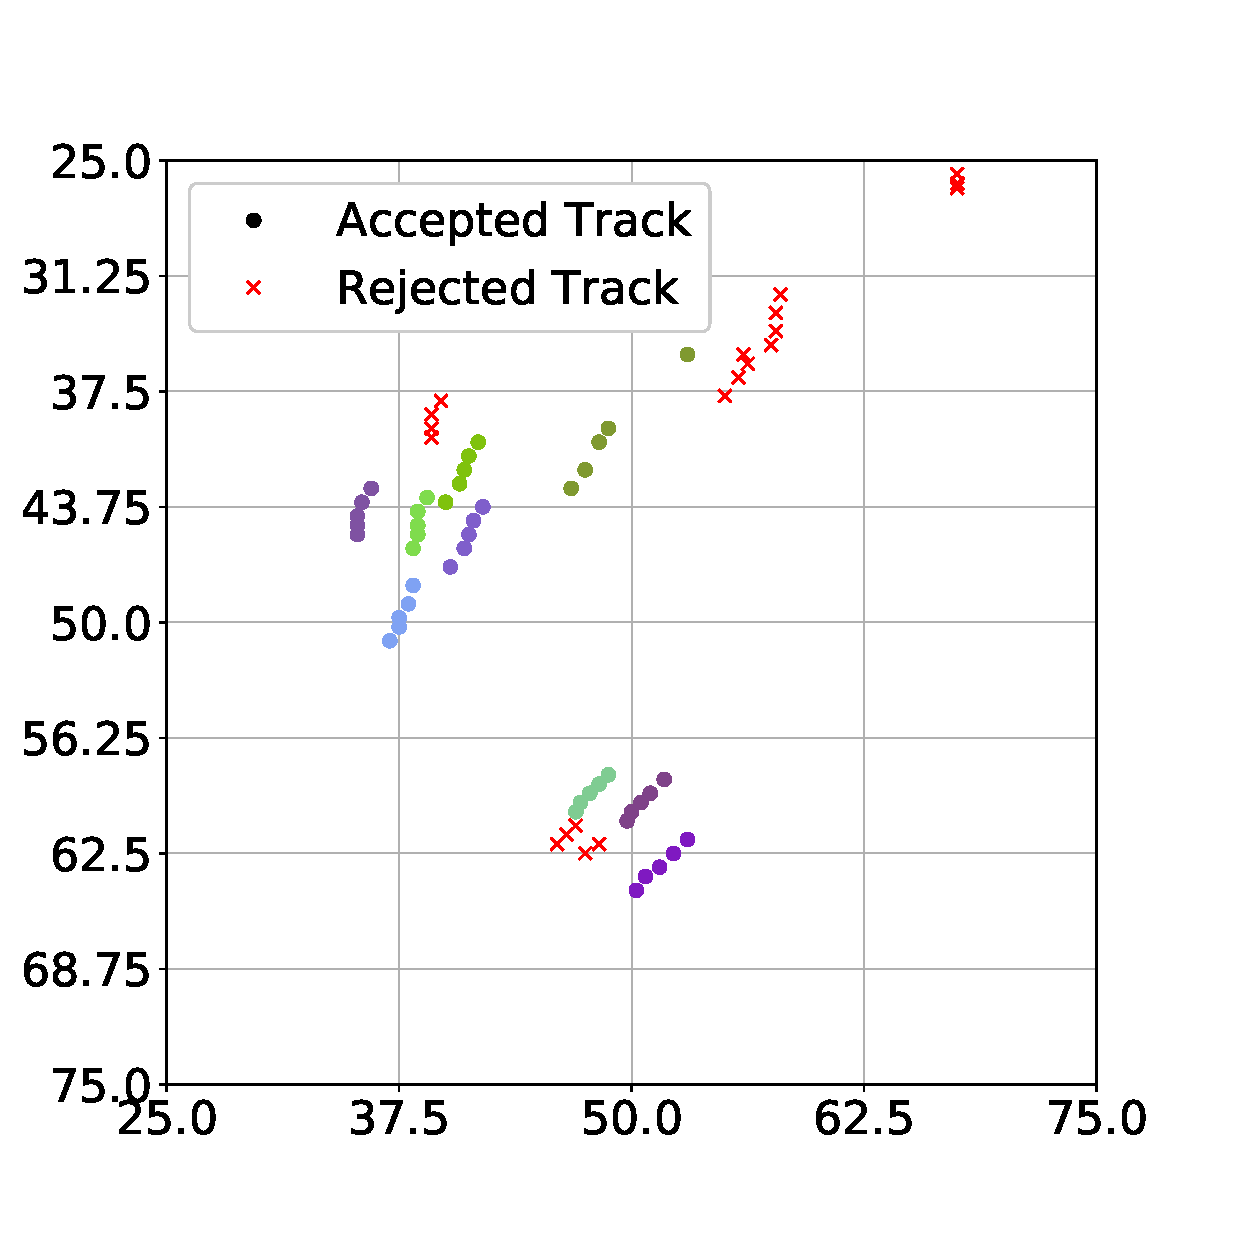
\includegraphics[width=0.8\textwidth,trim={0 0 5mm 0},clip]{displacement.eps}
	\caption{Tracks of patches over the time from the 13th June 2016, 19:20 UTC to 19:45 UTC of the DWD precipitation scan. The circles and crosses mark the centres of the tracked patches over the time period of 25 minutes. }
	\label{fig:displacement}
\end{figure}
\begin{figure}[!htbp]
	\centering
	\begin{tikzpicture}[dot/.style={circle,inner sep=1pt,fill,name=#1},
	extended line/.style={shorten >=-#1,shorten <=-#1},
	extended line/.default=0.2cm]
	\begin{axis}[
    scale only axis=true,
	axis lines=middle,
	xtick={0,1,...,5},
	ytick={0,1,...,5},
	grid=major,
	xmin=0,
	ymin=0,
	xmax=5.5,
	ymax=5.5
	]
	\node [dot=A] at (1,0) {};
	\node [dot=B] at (2,4) {};
	\node [dot=C] at (4,3) {};
	\node [dot=D] at (3,3) {};
	\node [dot=E] at (4,5) {};
	\node [dot=F] at (4,2) {};
	\coordinate (G) at (0,0);
	\coordinate (H) at (5,5);
	\draw (G) -- (H);
	\draw [red] ($(G)!(A)!(H)$) -- (A);
	\draw [red] ($(G)!(B)!(H)$) -- (B);
	\draw [red] ($(G)!(C)!(H)$) -- (C);
	%\draw [red] ($(G)!(D)!(H)$) -- (D);
	\draw [red] (E) -- ($(G)!(E)!(H)$);
	\draw [red] (F) -- ($(G)!(F)!(H)$);
	\draw [dotted] (A) -- (E);
	\end{axis}
	\end{tikzpicture}
	\caption{Example for the orthogonal distance regression. The black line is the line which is calculated by the orthogonal distance regression. The red lines show the distance from the points to their respective foot points on the line. The dotted line shows the distance between the first and the last point of the tracks.}
	\label{fig:orthogonaldist}
\end{figure}
%\FloatBarrier
\section{Bivariate Normal Densities}
\label{subsec:bivar}
After \cite{duda} a two dimensional Gaussian distribution, also called bivariate normal density, is defined in this section.
With $\sigma_x \cdot\sigma_y = \sigma_{xy}$, where $\sigma_{xy}$ is the covariance of $x$- and $y$ displacements, $\sigma_{x}$ is the standard deviation of the $x$ displacements and $\sigma_{y}$ is the standard deviation of the $y$ displacements, the correlation coefficient $\rho$ is defined by
\begin{equation}
	\rho = \dfrac{\sigma_{xy}}{\sigma_x\sigma_y}.
\end{equation}
With $\mu_x$ and $\mu_y$ as the means of all $x$- and $y$ displacements the bivariate normal density has the form
\begin{equation}
	\begin{multlined}
		p_{xy}(x,y)=\dfrac{1}{2\pi\sigma_x\sigma_y\sqrt{1-\rho^2}} \times \\ e^{-\dfrac{1}{2(1-\rho^2)}\bigg[\bigg(\dfrac{x-\mu_x}{\sigma_x}\bigg)^2-2\rho\bigg(\dfrac{x-\mu_x}{\sigma_x}\bigg)\bigg(\dfrac{y-\mu_y}{\sigma_y}\bigg)+\bigg(\dfrac{y-\mu_y}{\sigma_y}\bigg)^2\bigg]}.
	\end{multlined}
	\label{eq:bivariate}
\end{equation}
Now with eq. \ref{eq:bivariate} the $x$- and $y$ displacements from the tracks (Fig. \ref{fig:displacement}) are used to construct a bivariate normal density distribution. Here it is assumed that the $x$- and $y$ displacements are normal distributed.
\begin{figure}[!htbp]
	\centering
	\begin{tikzpicture}[
	declare function={mu1=2.65;},
	declare function={mu2=-1.61;},
	declare function={sigma1=0.74;},
	declare function={sigma2=1.05;},
	declare function={sigma12=-0.34;},
	declare function={rho=-0.438;},
	%[ 3.82178554  0.7623108 ]
	%[ 0.7623108   0.53510949]
	%[3.4090909090909092, -1.9545454545454546]
%	declare function={bivar(\ma,\sa,\mb,\sb,\corr)= 1/(2*pi*\sa*\sb) * exp( -((x-\ma)^2/(2*\sa^2)) - ((y-\mb)^2/(2*\sb^2)));}]
	declare function={bivar(\ma,\sa,\mb,\sb,\corr)= 1/(2*pi*sqrt(\sa)*sqrt(\sb)*sqrt(1-\corr^2)) * exp(-1/(2*(1-\corr^2))*((x-\ma)^2/sqrt(\sa)^2-2*\corr*(x-\ma)*(y-\mb)/(sqrt(\sa)*sqrt(\sb))+(y-\mb)^2/sqrt(\sb)^2));}]
	\begin{axis}[
	colormap name=whitered,
	width=12cm,
	view={45}{55},
	enlargelimits=false,
	scaled ticks = false,
	grid=major,
	domain=-5:5,
	y domain=-5:5,
	samples=41,
	xlabel=$x$,
	ylabel=$y$,
	zlabel={$P(x,y)$},
	colorbar,
	colorbar style={
		at={(1,0)},
		%ytick={0.05,0.1,0.15},
		%every ytick scale label/.style={at={(1,0)},anchor=south east},
		anchor=south west,
		height=0.2*\pgfkeysvalueof{/pgfplots/parent axis height},
		ylabel={$P(x,y)$},
		yticklabel style={
			%text width =2.5em,
			%align=right,
			scaled ticks = false,
			/pgf/number format/fixed,
			/pgf/number format/fixed zerofill,
			/pgf/number format/precision=2
			}
		}
	]
	\addplot3 [surf] {bivar(mu1,sigma1,mu2,sigma2,rho)};
	%\addplot3 [domain=-1:3,samples=51, samples y=0, thick, smooth] (x,3,{normal(mu1,sigma1)});
	%\addplot3 [domain=-1:3,samples=51, samples y=0, thick, smooth] (-1,x,{normal(mu2,sigma2)});
	
	\draw [black!80] (axis cs:-5,0,0) -- (axis cs:5,0,0);
	\draw [black!80] (axis cs:0,-5,0) -- (axis cs:0,5,0);
	\draw [blue!50] (axis cs:mu1,-5,0) -- (axis cs:mu1,5,0);
	\draw [blue!50] (axis cs:-5,mu2,0) -- (axis cs:5,mu2,0);
	\draw [blue!50] (axis cs:mu1,mu2,0) -- (axis cs:mu1,mu2,0.2);
	\node at (axis cs:mu1,mu2,0) [fill=blue,circle,scale=0.3] {};
	\node at (axis cs:mu1,mu2,0.2) [fill=blue,circle,scale=0.3,pin=15:{$P(\mu_x,\mu_y)$}] {};
	%\node at (axis cs:1.5,3,0.0) [pin=-15:$P(y)$] {};
	\end{axis}
	\end{tikzpicture}
	\caption{Bivariate Gaussian density constructed with following parameters: $\mu_x=2.65$, $\mu_y=-1.61$, $\sigma_x = 0.74$, $\sigma_y=1.05$ and $\rho = -0.44$. The parameters for the normal density have been derived from the tracks (Fig. \ref{fig:displacement}).}
	\label{fig:2dgauss}
\end{figure}
\section{Extrapolation}
\label{subsec:extrapolation}
Once the $x$- and $y$ displacements are estimated and evaluated, they are applied to the precipitation fields of the DWD and PATTERN radar to perform the prognosis. \\
The latest available DWD precipitation field is then simply globally advected by the mean $x$- and $y$ displacement vector estimated in section \ref{subsec:disdetect}. This method of a simple precipitation displacement is called Lagrangian persistence \citep{Germann}. Hereby it is assumed that the precipitation field does not change over the prognosis time and is merely advected horizontally. This obviously can lead to huge errors if the precipitation strengthens or weakens over time. Especially in convective situations this can cause faults in the prognosis. \\
The prognosis of the DWD precipitation fields is used as a boundary condition for the PATTERN precipitation fields. The PATTERN precipitation field is nested inside the DWD precipitation field (Fig. \ref{fig:radarOverview}). By nesting the PATTERN radar area inside the DWD radar area, the possible prognosis time is extended. When precipitation is on the boundary between the DWD and PATTERN radar and moves in the direction of the PATTERN radar area it is advected into the PATTERN radar area.\\
The PATTERN precipitation field is extrapolated by a different approach than the DWD precipitation field. Here the properties of the bivariate normal density (Fig. \ref{fig:2dgauss}) constructed in section \ref{subsec:bivar} are used. The displacement detection from section \ref{subsec:disdetect} shows that the past displacements of the precipitation fields are not unequivocally and do not deliver a clear value for using the past displacements for a prognosis of the future. This uncertainty is now used to perform a probabilistic precipitation forecast. \\
This is done by applying the bivariate normal density on the latest available PATTERN precipitation field. The procedure is similar to applying a Gaussian filter on an image to smooth the image. But here a shifted asymmetric bivariate normal density is used to apply a displacement and a smoothing onto the precipitation field. The smoothing represents the uncertainty in the displacement detection. A high uncertainty in the displacement detection, e.g. big differences within the distribution of the $x$- and $y$ displacements, leading to bigger variances and covariances which leads to a flatter bivariate normal density distribution. Higher certainties in the displacements detection obviously lead to a sharper density distribution. The means of the $x$- and $y$ displacements controls the direction and speed of the precipitation fields in the prognosis. This is visible in the Figures \ref{fig:2dgauss}, \ref{fig:extrapolation_t0} and \ref{fig:extrapolation_t1}. A mean of $\mu_x=2.65$ and $\mu_y=-1.61$ means that the average of the $x$- and $y$ displacements goes from the south-east to the north-west.\\
To apply the bivariate normal density distribution from Figure \ref{fig:2dgauss} on the precipitation field a kernel matrix (eq. \ref{eq:gausskernel}) from the values of the density distribution is constructed. 
\begin{equation}
K =	\begin{brmatrix}[1.3em]
0 & 0 & 0 & 0 & 0 & 0 & 0   & 0    	& 0 	& 0 	& 0 \\
0 & 0 & 0 & 0 & 0 & 0 & 0   & 0    	& 0	    & 0 	& 0 \\
0 & 0 & 0 & 0 & 0 & 0 & 0   & 0    	& 0		& 0 	& 0\\
0 & 0 & 0 & 0 & 0 & 0 & 0   & 0 	& 0 	& 0 	& 0 \\
0 & 0 & 0 & 0 & 0 & 0 & 0   & 0.01 	& 0 	& 0 	& 0 \\
0 & 0 & 0 & 0 & 0 & \textbf{0} & 0.02& 0.07 	& 0.03 	& 0 	& 0\\
0 & 0 & 0 & 0 & 0 & 0 & 0.02& 0.15 	& 0.14 	& 0.01 	& 0\\
0 & 0 & 0 & 0 & 0 & 0 & 0.01& 0.11	& 0.2 	& 0.04 	& 0\\
0 & 0 & 0 & 0 & 0 & 0 & 0   & 0.03	&   0.1 & 0.04 	& 0 \\
0 & 0 & 0 & 0 & 0 & 0 & 0   & 0    	&	0.01& 0.01 	& 0 \\
0 & 0 & 0 & 0 & 0 & 0 & 0   & 0    	&	0   & 0 	& 0
\end{brmatrix}
\label{eq:gausskernel}
\end{equation}The kernel shows how the new value for the pixel in the middle, depicted with a thick \textbf{0}, is calculated by the values around it weighted with the bivariate normal density. The filter is applied to every pixel in the image.\\
An example for this is shown in Figures \ref{fig:extrapolation_t0} and \ref{fig:extrapolation_t1}. Figure \ref{fig:extrapolation_t0} shows an example matrix with zeros and ones. Three quadrates with different sizes and a values of one are present in the matrix at the timestep $t=0$. Now the kernel  $K$ from eq. \ref{eq:gausskernel} is applied on the Figure \ref{fig:extrapolation_t0} to perform the extrapolation. In Figure \ref{fig:extrapolation_t1} it is shown how the kernel works. All pixels were shifted to the top left. By examining closely the pixel in the middle and comparing the shift of the maximum, you can observe that the maximum has moved two pixels to the top and three pixels to the left. This is caused by the maximum of the bivariate normal density at $\mu_x = 2.65$ and $\mu_y = -1.61$. Furthermore the smoothing of the kernel is also visible. The initial value of one of the pixel in the middle (Fig. \ref{fig:extrapolation_t0}) is now smoothed to the pixels around it (Fig. \ref{fig:extrapolation_t1}). \\
For the extrapolation of the PATTERN precipitation fields this procedure is now applied multiple times for the desired amount of timesteps. Since the temporal resolution of the PATTERN radar data is 30 seconds, each application of the kernel filtering represents a prognosis 30 seconds in the future. So a prognosis for 30 minutes would be achieved after applying the kernel filter 60 times.


%	0 & 0 & 0 & 0 & 0 & 0 & 0 & 0 & 0 & 0 & 0 \\
%0 & 0 & 0 & 0 & 0 & 0 & 0 & 0 &	0 & 0 & 0 \\
%0 & 0 & 0 & 0 & 0 & 0 & 0 & 0 & 0 & 0 & 0 \\
%0 & 0 & 0 & 0 & 0 & 0 & 0 & 0 &	0.01 & 0.01 & 0\\
%0 & 0 & 0 & 0 & 0 & 0 & 0 & 0.02 & 0.07 & 0.03 & 0\\
%0 & 0 & 0 & 0 & 0 & 0 & 0 & 0.09 & 0.19 & 0.04 & 0\\
%0 & 0 & 0 & 0 & 0 & 0 & 0.02 & 0.15 & 0.17 & 0.02 & 0 \\
%0 & 0 & 0 & 0 & 0 & 0 & 0.02 & 0.09 & 0.05 & 0 & 0 \\
%0 & 0 & 0 & 0 & 0 & 0 & 0.01 & 0.02 & 0 & 0 & 0\\
%0 & 0 & 0 & 0 & 0 & 0 & 0 & 0 &	0 & 0 & 0 
\begin{figure}[!htbp]
	\centering
	\begin{minipage}{0.48\textwidth}
		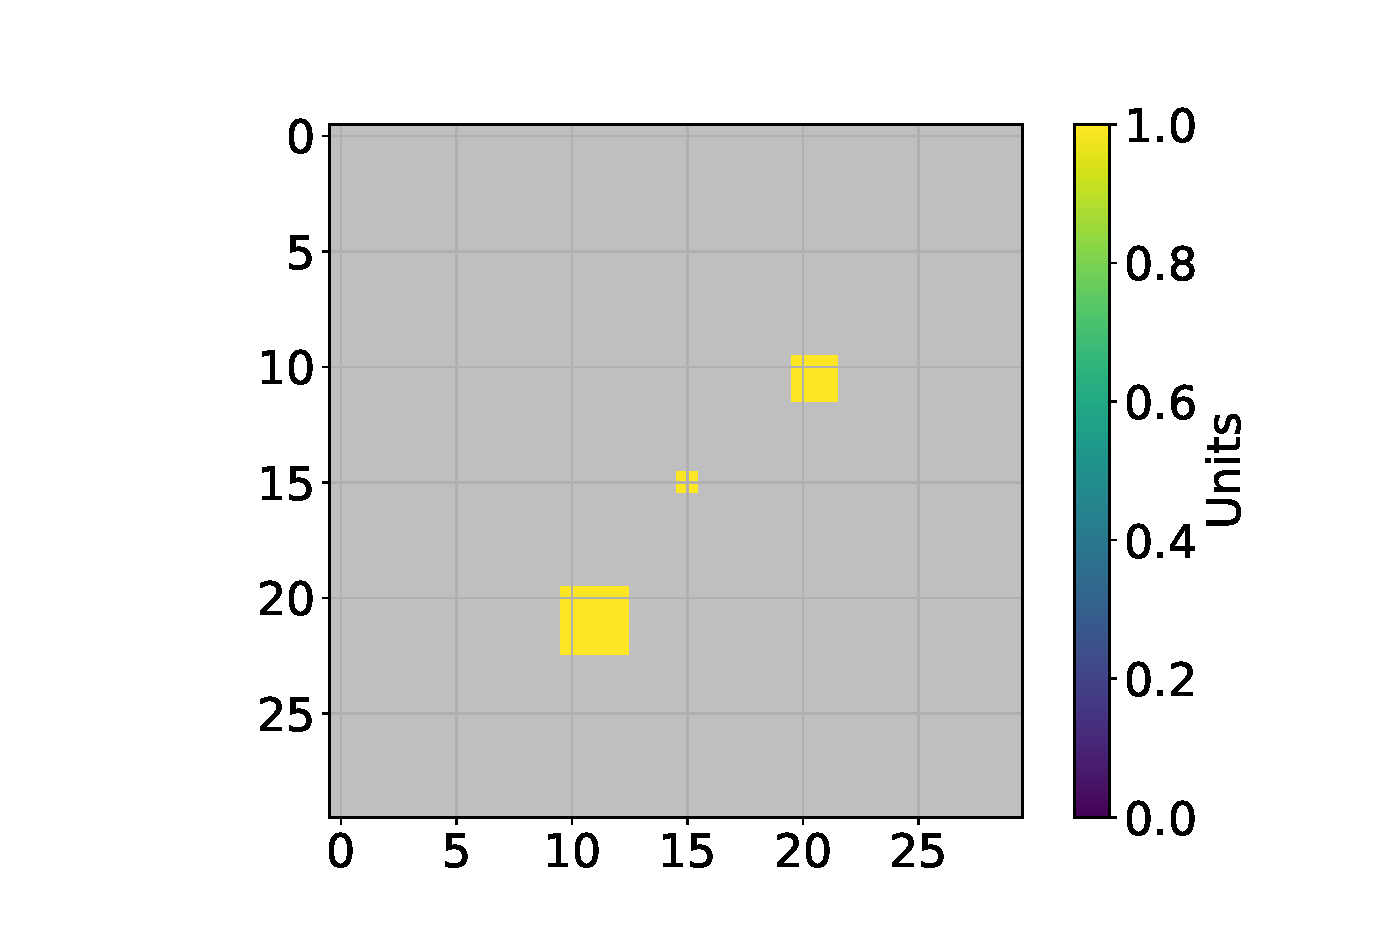
\includegraphics[width=\textwidth,trim={38mm 0 10mm 5mm},clip]{Extrapolation_t0.eps}
		\caption{Example plot with quadrates with sizes of 1px, 2px and 3px with a arbitrary value of 1, at timestep $t=0$. Gray colours show values of 0.}
		\label{fig:extrapolation_t0}
	\end{minipage}\hfill
	\begin{minipage}{0.48\textwidth}
		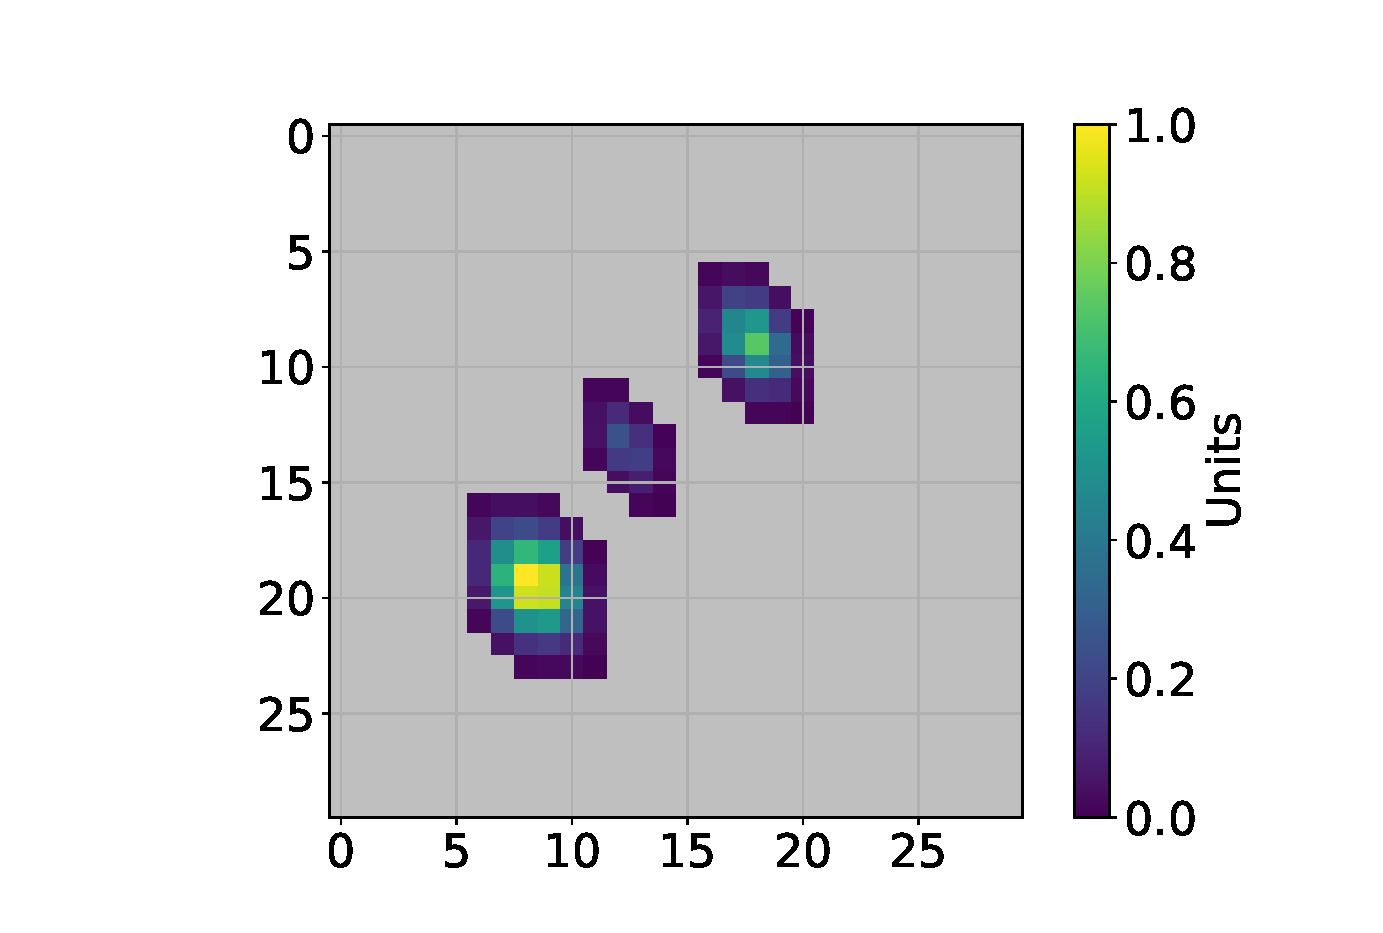
\includegraphics[width=\textwidth,trim={38mm 0 10mm 5mm},clip]{Extrapolation_t1.eps}
		\caption{Example plot where the pixels from Fig. \ref{fig:extrapolation_t0} are displaced and smoothed by eq. \ref{eq:gausskernel} at timestep $t=1$. Gray colours show values of 0.}
		\label{fig:extrapolation_t1}
	\end{minipage}
\end{figure}
\FloatBarrier

%\begin{figure}[h]
%	\centering
%	\begin{tikzpicture}[
%	declare function={mu1=2.65;},
%	declare function={mu2=-1.61;},
%	declare function={sigma1=0.74;},
%	declare function={sigma2=1.05;},
%	declare function={sigma12=-0.34;},
%	declare function={rho=-0.438;},
%	declare function={invgauss(\rnda,\rndb,\corr)=sqrt(-2*ln(\rnda))*sin(deg(2*pi*\rndb+asin(\corr)));}]%
%    \begin{axis}[
%	axis x line=center,
%	axis y line=center,
%	width=0.7\textwidth,
%	height=0.4\textwidth,
%	xtick={-6,-4,...,6,8},
%	ytick={-4,-2,...,2,4},
%	grid=major,
%	xmin=-6,
%	ymin=-4,
%	xmax=8,
%	ymax=4
%    ]
%	\fill (0,0) circle[radius=2pt];
%
%	\draw (1,0.5) node {$f_t(x,y)$};
%
%	\foreach \x in {0, ..., 24} {%A,mu,sigma,x
%		\pgfmathsetmacro{\xcoor}{rand}% x-coordinate
%		\edef\temp{
%			%\noexpand\coordinate (A) at ({gauss(1,0,1,\xcoor)},{gauss(1,0,1,\xcoor)});
%			\noexpand\coordinate (A) at ({invgauss(rnd,rnd,rho)*sigma1+mu1},{invgauss(rnd,rnd,rho)*sigma2+mu2});
%			\noexpand\draw (A) -- (0,0);	
%			\noexpand\fill (A) circle[radius=1pt];
%		}
%	\temp
%	}
%	%\draw (1.5,0.5) --(3,3);
%	%\fill (1.5,0.5) circle[radius=2pt];
%	\draw (6.75,-3) node {$f_{t+1}(x_s,y_s)$};
%
%    \end{axis}
%	\end{tikzpicture}
%	\caption{16 Drawn samples from the bivariate Gaussian Density function \ref{fig:2dgauss}}
%	\label{fig:importancesampling}
%\end{figure}


%\begin{equation}
%	f_{t+1}(x,y) = \frac{1}{N}\sum_{s=0}^{N} f_{t}(x_s,y_s)
%\end{equation}
%\section{Setting of Parameters}
%\label{subsec:param}
%Before the prognosis model can be started several parameters (Table \ref{tab:parameter}) need to be adjusted. The parameters control crucial parts of the model. The parameters 'gridded resolution of DWD and PATTERN' control the resolution of the Cartesian grid to which the radar data gets interpolated on. The train time represents the time how long the algorithm looks back in time to track the displacements of the precipitation fields. A train time of 30\,minutes for the DWD radar data represents 6 timesteps due the temporal resolution of 5\,minutes. The train time of 5\,minutes for the PATTERN radar data are equal to 10 timesteps, where each timestep has a temporal resolution of 30\,seconds. \\
%The 'maximum number of tracked patches' sets the maximum number of tracked patches. The number of patches is also limited by the amount of precipitation pixels inside the radar field. If no more pixels above 0.5\,mmh$^{-1}$, threshold determined by the parameter 'rain rate threshold', can be found no more patches are created. The parameter 'distance threshold' determines how far away the centre of the patches are allowed to move from the centre of the radar area. This is introduced to reduce unwanted interactions of the displacement detection with the border of the radar area. For the PATTERN and the DWD radar this centre is the PATTERN radar location. \\
%For this prognosis model the maximum speed of clouds is assumed to be around 80\,kmh$^{-1}$(\textbf{Reference needed?}), so the 'speed threshold' is set to 80\,km$^{-1}$. This threshold limits the distance of single displacement. For the DWD radar this means the maximum distance of a single displacement is limited to approx. 6000\,m, for the PATTERN radar the maximum distance is approx. 1000\,m. The parameter 'lead time' sets the time for what duration the prognosis should run. \\
%The 'minimum distance between maxima' determines the distance between maxima for the initial maxima detection (section \ref{subsec:disdetect}). This is set to 3000\,m for both radars and is implemented to evenly spread the patches over the total radar area. Motivated by the speed threshold for clouds the 'displacement detection range for DWD and PATTERN' is set to 6000\,m and 1000\,m. \\
%The 'edge length of the patches for DWD and PATTERN' is set to 12000\,m and 2000\,m. This results in patch sizes of 12000\,m x 12000\,m for DWD and 2000\,m x 2000\,m for PATTERN. The 'ODR squared distance threshold' determines how far single displacements are allowed to stray from their respective regression line. With a higher value for this threshold higher variations are allowed. This parameter is relevant for the displacement evaluation in section \ref{subsec:disdetect}.
%\begin{table}[ht]
%	\centering
%	\caption[]{List of parameters for the prognosis algorithm.}
%	\label{tab:parameter}
%	\begin{tabular}{|l|l|l|}
%		\hline
%		Name of parameter &Value & Unit\\\hline
%		Gridded resolution of DWD & 250 & meters\\
%		Gridded resolution of PATTERN & 100 & meters\\
%		Train time of DWD & 30 & minutes\\
%		Train time of PATTERN & 5 & minutes\\
%		Maximum number of tracked patches DWD& 20 & number\\
%		Maximum number of tracked patches PATTERN& 20 & number\\
%		Distance threshold for DWD & 50000 & meters\\
%		Distance threshold for PATTERN &  19000 & meters\\
%		Rain rate threshold & 0.5 & mmh$^{-1}$ \\
%		Speed threshold & 80 & kmh$^{-1}$  \\
%		Lead time  & 60 & minutes \\
%		%Azimuth correction for PATTERN & -5 & degrees \\
%		Minimum distance between maxima & 3000 & meters \\
%		Displacement detection range for DWD & 6000 & meters\\
%		Displacement detection range for PATTERN & 1000 & meters\\
%		Edge length of patches for DWD & 12000 & meters\\
%		Edge length of patches for PATTERN & 2000 & meters\\
%		ODR squared distance threshold & 0.5 & fraction \\\hline
%		%Minimum kernel filter size & 20x20 & pixels \\\hline
%	\end{tabular}
%\end{table}
\FloatBarrier
\section{Evaluation Methods for Binary Events}
The occurrence of precipitation can be regarded as a binary event. Either it rains, represented with \textbf{Yes} or a '1', or it does not rain, represented with \textbf{No} or a '0'. So testing if a nonprobabilistic prognosis of an event is correct is straightforward. By comparing the binary representations of the forecast and the observation four scenarios are possible (Fig. \ref{fig:contingency}). With the contingency table the further evaluation of a nonprobabilistic forecast becomes possible. Generally speaking a greater number of \textit{hits} and \textit{correct rejection} events indicates a better forecast. More \textit{misses} and \textit{false alerts} indicate a worse forecast.
\begin{figure}[!htbp]
\centering
	\begin{tikzpicture}[
		box/.style={draw,rectangle,minimum size=2cm,text width=1.5cm,align=center}]
		\matrix (conmat) [row sep=.1cm,column sep=.1cm] {
		\node (tpos) [box,
		label=left:\textbf{Yes},
		label=above:\textbf{Yes},
		] {a};
		&
		\node (fneg) [box,
		label=above:\textbf{No},
		label=right:a+b] {b};
		\\
		\node (fpos) [box,
		label=left:\textbf{No},
		label=below:a+c] {c};
		&
		\node (tneg) [box,
		label=right:c+d,
		label=below:b+d,
		label={[xshift=1.575cm,yshift=-2.55cm]\textbf{n}}] {d};
		\\
		};
		\node [rotate=90,left=.05cm of conmat,anchor=center,text width=1.5cm,align=center] {\textbf{Forecast}};
		\node [above=.05cm of conmat] {\textbf{Observation}};
	\end{tikzpicture}
	\caption[Contingency Table for Nonprobabilistic Forecasts of Binary Events]{Contingency table for nonprobabilistic forecasts of binary events. Four different scenarios are possible. In case of the scenario $a$, where both the observation and the forecast show a \textbf{Yes}, the forecast was successful. This pair is called \textit{hit}. The other desirable outcome of the forecast is an observation and forecast of a \textbf{No}. This is represented with a $d$ and called \textit{correct rejection}. In the $b$ scenario, called \textit{false alert}, the event was forecast to occur but did not happen. In the last case $c$ the event was not forecast but did occur. This scenario is called \textit{miss}. The marginal totals are shown on the bottom and right of the boxes. These indicate how often each of the events were forecast and observed. The total number of forecasts is $n$. After \cite{Wilks}.}
	\label{fig:contingency}
\end{figure}\\
Evaluating probabilistic forecasts is less intuitive than evaluating nonprobabilistic forecasts. Unless the probability forecast shows values of either 0.0 or 1.0, there is no right or wrong for a single forecast. 
\label{subsec:eval}
\citep{Wilks}
\subsection{Brier Score}
One possible measure for evaluating a probabilistic forecast is the scalar Brier score. The Brier score is essentially the mean square error (MSE) in probability space. To calculate the Brier Score the observation is $o_1 = 1$ if the event occurs and $o_2 = 0$ if the observation does not occur. The Brier Score averages the squared differences between pairs of forecast probabilities and binary observations:
\begin{equation}
	BS = \frac{1}{n}\sum_{k=1}^{n}(y_{k}-o_{k})^{2}
	\label{eq:brier}
\end{equation}
Here the index $k$ denotes the numbering of the total number $n$ of forecast-observation pairs. The forecast probability is described by $y_k$. The Brier score has values in the range from 0 to 1. A lower Brier score indicates a better forecast and a perfect forecast is represented by a Brier score of 0. 
\subsection{Reliability Diagram}
Reliability diagrams are graphs of the full joint distribution of forecasts and observations for probability forecasts of a binary event (Figure \ref{fig:reliability}). The reliability diagram shows how often a forecast probability actually occurred \citep{Wilks}.%% formulierung
%(0, 0.3) (0.1, 0.1) (0.2, 0.05) (0.3, 0.08) (0.4, 0.07) (0.5, 0.1) (0.6, 0.08) (0.7, 0.02) (0.8, 0.05) (0.9, 0.05) (1,0.15)
\begin{table}[!htbp]
	\centering
	\begin{tabular}{cccccccccccc}
		\hline
		$y_i$ & 0.0 & 0.1 &0.2 &0.3 &0.4 &0.5 &0.6 &0.7 &0.8 &0.9 &1.0\\\hline
		$p(o_1|y_i)$ & .03&.09&.17&.26&.33&.49&.64&.72&.82&.88&.95\\
		$p(y_i)$& .29&.11&.10&.08&.07&.09&.09&.02&.05&.05&.10\\\hline
	\end{tabular}
	\caption[]{Verification data for a probabilistic forecast of a binary event. For the different forecast probabilities, $y_i$, the conditional probability $p(o_1|y_i)$ indicates the relative frequency of a positive  event. The marginal probabilities $p(y_i)$ show the relative frequencies with which each forecast probability occurred. The sample climatological relative frequency is 0.38.}
	\label{tab:verification}
\end{table}\\
To create a reliability diagram the forecasted probabilities are binned into probability bins (Table \ref{tab:verification}), $y_i$ shows the centres of the probability bins. For the exemplary data shown in Table \ref{tab:verification} this means that in 29\% of the forecasted probabilities a probability $y_i$ of 0.0 is present. In 3\% of the forecasted probabilities of $y_i = 0.0$ this resulted in a positive event ($p(o_1|y_0) = 0.03$). A perfect forecast would show a conditional probability $p(o_1|y_i) = 0.0$ for a forecast probability of $y_i = 0.0$. This means in the probability bin of $y_i=0.0$ the exemplary forecast predicted more positive events than actually occurred. In case of the forecast probability of $y_i = 0.4$, the forecast only shows an observed relative frequency $p(o_1|y_i)$ of 0.33. In the $y_i = 0.4$ probability bin the forecast predicted less positive events than actually occurred.\\
A perfect forecast is defined by conditional event relative frequency being equal to the forecast probability ($p(o_1|y_i) \approx y_i$), so that the calibration function would lie close to the dotted 1:1 line in Figure \ref{fig:reliability}. Small deviations from the line can be caused by sampling variability.
\begin{figure}[!htbp]
	\centering
	\begin{tikzpicture}[dot/.style={circle,inner sep=1.5pt,fill,name=#1},
	extended line/.style={shorten >=-#1,shorten <=-#1},
	extended line/.default=0.2cm]
	\begin{axis}[
    scale only axis=true,
    axis lines=middle,
	axis line style={-},
	xtick={0,0.2,...,1.0},
	ytick={0,0.2,...,1.0},
    x label style={at={(axis description cs:0.5,-0.1)},anchor=north},
	y label style={at={(axis description cs:-0.1,.5)},rotate=90,anchor=south},
	xlabel={Forecast probability},
	ylabel={Observed relative frequency},
	grid=major,
    major grid style={line width=.2pt,draw=gray!50},
    grid style={line width=.1pt, draw=gray!10},
	xmin=0,
	ymin=0,
	xmax=1,
	ymax=1
	]
	\node [dot=A] at (0,0.03) {};
	\node [dot=B] at (0.1,0.09) {};
	\node [dot=C] at (0.2,0.17) {};
	\node [dot=D] at (0.3,0.26) {};
	\node [dot=E] at (0.4,0.33) {};
	\node [dot=F] at (0.5,0.49) {};
	\node [dot=G] at (0.6,0.64) {};
	\node [dot=H] at (0.7,0.72) {};
	\node [dot=I] at (0.8,0.82) {};
	\node [dot=J] at (0.9,0.88) {};
	\node [dot=K] at (1,0.95) {};
	\draw (A)--(B)--(C)--(D)--(E)--(F)--(G)--(H)--(I)--(J)--(K);
	\draw[dotted] (0,0) -- (1,1);
	\node at (0.4,0.62) [text width=5cm] {Perfect reliability};
	\draw [->] (0.25,0.58)--(0.36,0.37);
	\draw (axis cs: 0.759,0.25)node{\usebox{\mybox}};
	\end{axis}
	\end{tikzpicture}
	\caption[Reliability Diagram]{Reliability diagram for an example forecast. The dots show the observed relative frequency of the occurrence of precipitation. The black line shows the calibration function. The dotted line shows a perfect forecast. In the histogram in the bottom right the probability frequency distribution of the example forecast is shown. Figure created after \cite{Wilks}.}
	\label{fig:reliability}
\end{figure}\\
By comparing the calibration function to the 1:1 line of the perfect forecast, strengths or weaknesses of the probabilistic prognosis can be identified. When the calibration function lies on the right side of the 1:1 line, the forecasts are consistently too large compared to the conditional event relative frequencies (Figure \ref{fig:calibration}a). In case of a precipitation forecast the prognosis has a wet bias. A calibration function, which forecasts are consistently too small relative to the observed relative frequency, lies on the left side of the 1:1 line (Figure \ref{fig:calibration}b). This indicates that the forecast is underforecasting and has a dry bias.
\begin{figure}[!htbp] 
	\begin{subfigure}{0.5\textwidth}
		\centering
		\begin{tikzpicture}[dot/.style={circle,inner sep=3pt,fill,name=#1},
		extended line/.style={shorten >=-#1,shorten <=-#1},
		extended line/.default=0.2cm,scale=0.5]
		\begin{axis}[
		scale only axis=true,
		axis line style={-},
		xtick={0,1.0},
		ytick={0,1.0},
		tick label style={font=\Huge,outer sep=3pt},
		label style={font=\Huge},
		x label style={at={(axis description cs:0.5,-0.1)},anchor=north},
		y label style={at={(axis description cs:-0.1,.5)},anchor=south},
		ylabel={$p(o_1,y)$},
		xlabel={$y$},
		xmin=0,
		ymin=0,
		xmax=1,
		ymax=1
		]
		\node [dot=A] at (0.15,0.05) {};
		\node [dot=B] at (0.3,0.18) {};
		\node [dot=C] at (0.45,0.35) {};
		\node [dot=D] at (0.6,0.45) {};
		\node [dot=E] at (0.75,0.62) {};
		\node [dot=F] at (0.9,0.75) {};
		\draw[ultra thick] (A)--(B)--(C)--(D)--(E)--(F);
		\draw[ultra thick,loosely dotted] (0,0) -- (1,1);
		\end{axis}
		\end{tikzpicture}
		\subcaption{Overforecasting (wet bias)} 
	\end{subfigure}
	\,
	\begin{subfigure}{0.5\textwidth}
		\centering
		\begin{tikzpicture}[dot/.style={circle,inner sep=3pt,fill,name=#1},
		extended line/.style={shorten >=-#1,shorten <=-#1},
		extended line/.default=0.2cm,scale=0.5]
		\begin{axis}[
		scale only axis=true,
		axis line style={-},
		xtick={0,1},
		ytick={0,1},
		tick label style={font=\Huge,outer sep=3pt},
		label style={font=\Huge},
		x label style={at={(axis description cs:0.5,-0.1)},anchor=north},
		y label style={at={(axis description cs:-0.1,.5)},anchor=south},
		ylabel={$p(o_1,y)$},
		xlabel={$y$},
		xmin=0,
		ymin=0,
		xmax=1,
		ymax=1
		]
		\node [dot=A] at (0.10,0.25) {};
		\node [dot=B] at (0.25,0.43) {};
		\node [dot=C] at (0.4,0.54) {};
		\node [dot=D] at (0.55,0.63) {};
		\node [dot=E] at (0.7,0.8) {};
		\node [dot=F] at (0.85,0.94) {};
		\draw[ultra thick] (A)--(B)--(C)--(D)--(E)--(F);
		\draw[ultra thick,loosely dotted] (0,0) -- (1,1);
		\end{axis}
		\end{tikzpicture} 
		\subcaption{Underforecasting (dry bias)} 
	\end{subfigure} 
	\vskip\baselineskip
	\begin{subfigure}{0.5\textwidth}
		\centering
		\begin{tikzpicture}[dot/.style={circle,inner sep=3pt,fill,name=#1},
		extended line/.style={shorten >=-#1,shorten <=-#1},
		extended line/.default=0.2cm,scale=0.5]
		\begin{axis}[
		scale only axis=true,
		axis line style={-},
		xtick={0,1},
		ytick={0,1},
		tick label style={font=\Huge,outer sep=3pt},
		label style={font=\Huge},
		x label style={at={(axis description cs:0.5,-0.1)},anchor=north},
		y label style={at={(axis description cs:-0.1,.5)},anchor=south},
		ylabel={$p(o_1,y)$},
		xlabel={$y$},
		xmin=0,
		ymin=0,
		xmax=1,
		ymax=1
		]
		\node [dot=A] at (0.15,0.2) {};
		\node [dot=B] at (0.3,0.27) {};
		\node [dot=C] at (0.45,0.34) {};
		\node [dot=D] at (0.6,0.47) {};
		\node [dot=E] at (0.75,0.45) {};
		\node [dot=F] at (0.9,0.60) {};
		\draw[ultra thick] (A)--(B)--(C)--(D)--(E)--(F);
		\draw[ultra thick,loosely dotted] (0,0) -- (1,1);
		\end{axis}
		\end{tikzpicture}
		\subcaption{Poor resolution (overconfident)} 
	\end{subfigure}
	\,
	\begin{subfigure}{0.5\textwidth}
		\centering
		\begin{tikzpicture}[dot/.style={circle,inner sep=3pt,fill,name=#1},
		extended line/.style={shorten >=-#1,shorten <=-#1},
		extended line/.default=0.2cm,scale=0.5]
		\begin{axis}[
		scale only axis=true,
		axis line style={-},
		xtick={0,1},
		ytick={0,1},
		tick label style={font=\Huge,outer sep=3pt},
		label style={font=\Huge},
		x label style={at={(axis description cs:0.5,-0.1)},anchor=north},
		y label style={at={(axis description cs:-0.1,.5)},anchor=south},
		ylabel={$p(o_1,y)$},
		xlabel={$y$},
		xmin=0,
		ymin=0,
		xmax=1,
		ymax=1
		]
		\node [dot=A] at (0.10,0.02) {};
		\node [dot=B] at (0.25,0.1) {};
		\node [dot=C] at (0.4,0.30) {};
		\node [dot=D] at (0.55,0.6) {};
		\node [dot=E] at (0.7,0.85) {};
		\node [dot=F] at (0.85,0.95) {};
		\draw[ultra thick] (A)--(B)--(C)--(D)--(E)--(F);
		\draw[ultra thick,loosely dotted] (0,0) -- (1,1);
		\end{axis}
		\end{tikzpicture} 
		\subcaption{Good resolution (underconfident)} 
		
	\end{subfigure}%% 
	
	\caption[Example Calibration Functions]{Examples for characteristic calibration functions. The calibration functions $p(o_1,y)$ are shown for probabilities $y$ of different forecasts of exemplary data. Figure created after \citep{Wilks}.}
	\label{fig:calibration}
\end{figure}\\
The calibration curve in Figure \ref{fig:calibration}c depicts the characteristics of forecasts showing poor resolution. This means the observed relative frequencies $p(o_1|y_i)$ depend only weakly on the forecast and are close to the climatological probability \citep{Wilks}.
%TODO Hier noch über die calibration curve mit good resolution in figure d.
\subsection{ROC Skill Score}
The relative operating characteristic (ROC) is a measure of the quality of probability forecasts that compares the false alarm rate to the hit rate for specific probability bins (Figure \ref{fig:roc}). Following the nomenclature from the contingency table in Figure \ref{fig:contingency} the false alarm rate (FAR) and hit rate (HR) for a deterministic forecast are calculated by:
\begin{equation}
	FAR = \frac{b}{b + d}
	\label{eq:FAR}
\end{equation}
and
\begin{equation}
	HR = \frac{a}{a + c}.
	\label{eq:HR}
\end{equation}
The false alarm rate has values between 0 and 1, where 0 is desirable and shows how often an event was forecast to occur but did not occur. The hit rate also has values between 0 and 1, where 1 is desirable and indicates how often an event was forecast to occur and did occur.
\begin{figure}[!htbp]
	\centering
	\begin{tikzpicture}[dot/.style={circle,inner sep=1.5pt,fill,name=#1},
	extended line/.style={shorten >=-#1,shorten <=-#1},
	extended line/.default=0.2cm]
	\begin{axis}[
	scale only axis=true,
	axis line style={-},
	xtick={0,0.2,...,1},
	ytick={0,0.2,...,1},
	x label style={at={(axis description cs:0.5,-0.1)},anchor=north},
	y label style={at={(axis description cs:-0.1,.5)},anchor=south},
	ylabel={Hit rate},
	xlabel={False alarm rate},
	grid=major,
	major grid style={line width=.2pt,draw=gray!50},
	grid style={line width=.1pt, draw=gray!10},
	xmin=0,
	ymin=0,
	xmax=1,
	ymax=1
	]
	\node [dot=A] at (0,0) {};
	\node [label=right:{90\%},dot=B] at (0.03,0.4) {};
	\node [label=right:{80\%},dot=C] at (0.06,0.6) {};
	\node [label=below right:{70\%},dot=D] at (0.1,0.78) {};
	\node [label=above left:{60\%},dot=E] at (0.12,0.82) {};
	\node [label=above:{50\%},dot=F] at (0.15,0.85) {};
	\node [label=below:{40\%},dot=G] at (0.3,0.89) {};
	\node [label=below:{30\%},dot=H] at (0.45,0.91) {};
	\node [label=below:{20\%},dot=I] at (0.65,0.95) {};
	\node [label=below:{10\%},dot=J] at (0.75,0.97) {};
	\node [dot=K] at (1,1) {};
	\draw (A)--(B)--(C)--(D)--(E)--(F)--(G)--(H)--(I)--(J)--(K);
	
	\node [dot=BA] at (0,0) {};
	\node [dot=BB] at (0.1,0.25) {};	
	\node [dot=BC] at (0.16,0.4) {};	
	\node [dot=BD] at (0.24,0.6) {};
	\node [dot=BE] at (0.27,0.64) {};
	\node [dot=BF] at (0.3,0.67) {};
	\node [dot=BG] at (0.4,0.7) {};
	\node [dot=BH] at (0.52,0.75) {};	
	\node [dot=BI] at (0.7,0.85) {};	
	\node [dot=BJ] at (1,1) {};	
	
	\draw[fill=black!10,fill opacity = 0.65] (BA.center)--(BB.center)--(BC.center)--(BD.center)--(BE.center)--(BF.center)--(BG.center)--(BH.center) --(BI.center) -- (BJ.center)-- (1,0)--cycle;
	\node at (0.45,0.55) [text width=3cm] {Random\\forecast};
	\draw [->] (0.34,0.49)--(0.37,0.38);
	\draw[dashed] (0,0) -- (1,1);
	\node (dummy) at (1,0) {};
	\node [draw] at (0.6,0.3) {ROC Area};
	\end{axis}
	\end{tikzpicture}
	\caption[ROC Diagram]{ROC diagram for exemplary data. The solid dots represent pairs of false alarm rate and hit rate.} 
	\label{fig:roc}
\end{figure}
The ROC is derived from the comparison between two probability distributions. One distribution represents the evidence strength associated with the occurrence of the event and the other distribution represents the non-event distribution \citep{Kharin2003}. From these two distributions the false alarm rate and the hit rate are obtained as a function of probability. To calculate the ROC skill score for a probabilistic forecast the forecast is divided into probability intervals. Frequently used intervals are 10\% bins and are also used in this thesis. With a contingency table (Figure \ref{fig:contingency}) the false alarm rate and hit rate are calculated for each probability bin. For example the hit rate for the 70\% probability bin is the sum of hits (represented with $a$ in Figure \ref{fig:contingency})  above 70\% divided by total number of occurrences ($a + c$ in Figure \ref{fig:contingency}).\\
After \cite{Wilks} the ROC skill score SS$_\text{ROC}$ is defined as the area \text{A} under a ROC curve (grey area in Figure \ref{fig:roc}) and is calculated by:
\begin{equation}
	\text{SS}_{\text{ROC}} = 2\,\text{A} -1
	\label{eq:roc}
\end{equation}
A ROC curve for a perfect forecast passes through the upper-left corner at the point (0,1) and has a $\text{SS}_{\text{ROC}} = 1$, since the area under a ROC curve of a perfect forecast includes the complete unit square. The area under a ROC curve of a random forecast encompasses the half of the unit square A $ = 0.5$ and has a $\text{SS}_{\text{ROC}} = 0.5$.

\chapter{Results and Discussion}
% beispiel für problem bei intensivierung result = prognosis([2016,6,13,19,20,60],0) dwd, ca. 20 zeitschritt, großer sprung aufgrund von intensivierung und abschwächung einer regen wolke

\chapter{Conclusion and Outlook}
\chapter{Acknowledgement}
\bibliography{References}
\chapter{Eidesstattliche Versicherung}
Ich versichere an Eides statt, dass ich diese Arbeit selbstständig verfasst und keine anderen als die angegebenen Hilfsmittel benutzt habe. Insbesondere habe ich keine im Literaturverzeichnis nicht genannten Internet-Quellen benutzt. Diese Arbeit habe ich vorher nicht in einem anderen Prüfungsverfahren eingereicht und die eingereichte schriftliche Fassung entspricht der Fassung auf dem elektronischen Speichermedium. Ich stimme einer Veröffentlichung dieser Arbeit zu.
\\
\\
\\
\\
\\
Simon Michel\\
Hamburg, \today
\end{document}

